\chapter{肌肉驱动的跑步} \label{chap:chap12}


我尽量减少双脚接触地面的时间。
\begin{flushright}
	——杰西$\cdot$欧文斯
\end{flushright}

\begin{figure}[!htb]
	\centering
	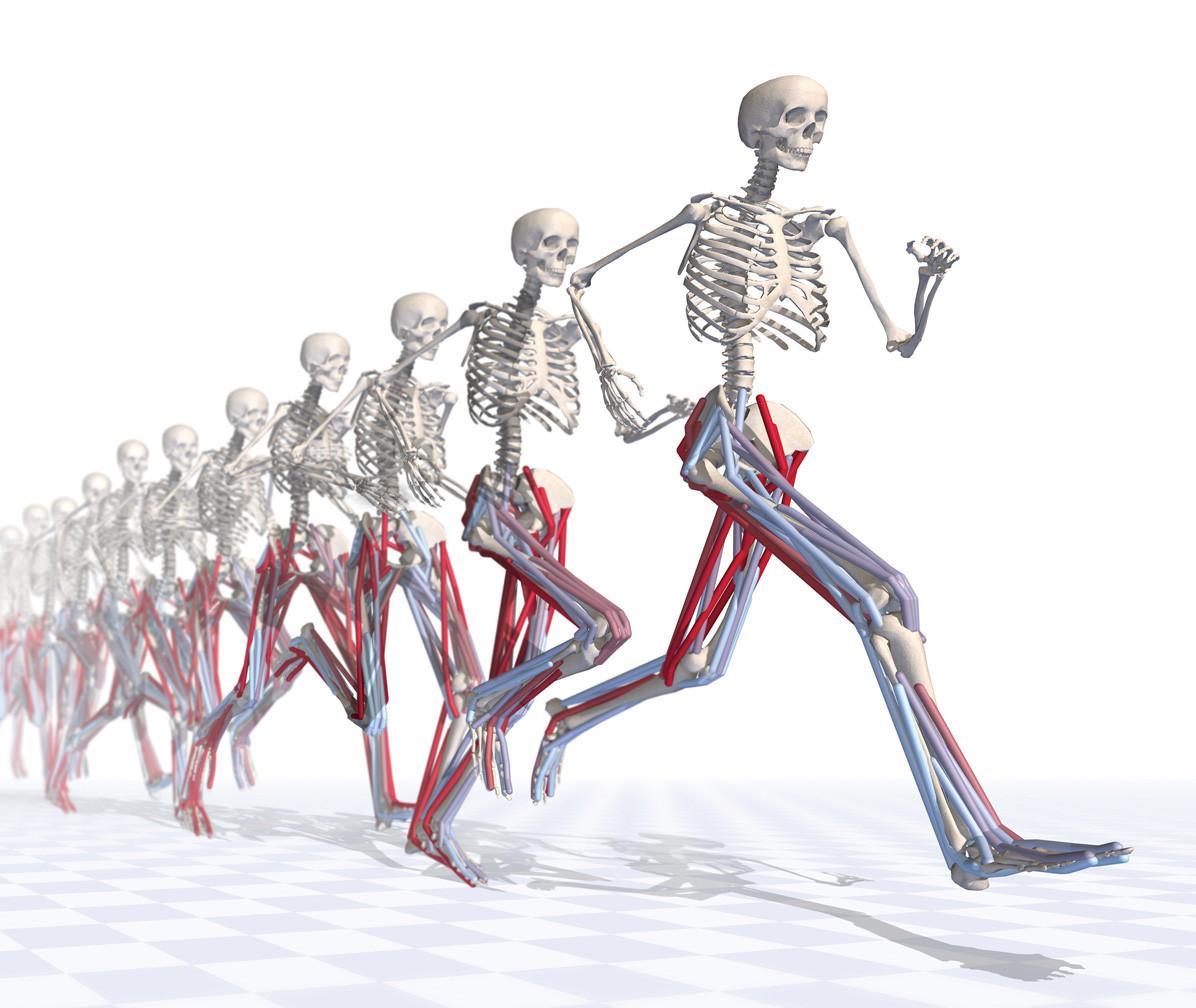
\includegraphics[width=1.0\linewidth]{chap12/12_0}
	% 加星号(*)表示不加编号
	\caption*{ \label{fig:12_0}}
\end{figure}


早在两百万年前,人类祖先就开始以跑步作为交通工具。
如今,我们跑步是为了锻炼,是为了赶时间,也是为了热爱跑步。
我们并非地球上跑得最快的动物——跑得最快的动物是猎豹,它的最高速度约为每秒30米,远超人类短跑运动员的两倍。
然而,我们以及我们祖先的身体特征,让我们成为优秀的长跑运动员。


每年,人马马拉松赛都会考验我们的长跑能力。
这项赛事的起源是威尔士酒吧老板戈登$\cdot$格林(Gordon Green)与一位朋友就马和人谁跑得更快而发生争执。
格林认为,人类可以在长距离上击败马,并于1980年发起了马拉松赛以解决这一分歧。
比赛距离为22英里(约35公里),略短于正式的马拉松。
二十多年来,骑马者一直战胜人类跑步者。
但在2004年,一位名叫休$\cdot$洛布(Huw Lobb)的英国男子以2小时5分19秒的成绩完成了比赛,比最快的马快了约2分钟。
3 年后,另外两名男子也超越了他们的四足竞争对手。


人类跑步最重要的特征之一,就是我们能够高效地长距离移动的弹跳步态。
在跑步过程中,身体重心在站立阶段的前半段会减慢并降低,从而将弹性能量储存在肌肉和肌腱中。
在站立阶段的后半段,储存的能量会从这些组织中释放出来,加速重心向前向上飞跃。
这一非凡的壮举发生在足部与地面接触的200至300毫秒内,每一步都发生着。


对质心轨迹和地面反作用力的分析表明,弹性能量的储存和释放对于高效跑步至关重要(Cavagna 等人,1976 年)。
这一发现促使研究人员开发出将所有下肢肌肉用单个弹簧表示的跑步模型(图 3.5)。
这些简单的质量弹簧模型为了解跑步动力学提供了宝贵的见解,并使研究人员能够调整跑道以提高跑步速度(图 3.10)。
虽然质量弹簧模型为研究跑步动力学提供了宝贵的理论框架,但这些模型并非旨在描述单个肌肉的动作。
然而,研究跑步过程中的肌肉动作对于了解肌肉结构和肌腱柔顺性如何影响跑步表现以及为设计提高跑步速度和效率的训练计划和技术提供信息至关重要。


肌肉驱动的跑步模拟提供了这种更深入的视角。
它们补充了我们在第~\ref{chap:chap3}~章讨论的质量弹簧模型,提供了一种系统的方法来估算肌肉力量及其对地面反作用力的贡献。
在本章中,我们将看到质量弹簧模型只是故事的一部分。
没错,人类之所以能高效奔跑,部分原因是跟腱储存了弹性能。
但这种肌腱的弹性也使得附着的肌肉能够更高效地运作。
与直觉相反,当我们加快步伐,从快走过渡到慢跑时,跖屈肌的收缩速度会变慢,从而使肌肉能够更有效地产生力量。
这种现象是质量弹簧模型无法预测的。


本章探讨肌肉在跑步过程中如何影响地面反作用力,进而影响身体重心的支撑和推进力。
我们将研究肌肉在典型的4米/秒长跑速度下的活动情况,并描述肌肉激活、地面反作用力以及肌肉对支撑和推进力的贡献如何随着跑步速度的变化而变化——从略高于2米/秒的步行到跑步的过渡速度到5米/秒的快跑。
我们还将了解短跑与低速跑步的区别,并探讨跑步界一个备受争议的话题:前脚掌和后脚掌着地方式的区别。
最后,我们将研究科技如何提升跑步表现。


\section{构建和测试跑步模拟}

为了研究跑步过程中的肌肉动作,Sam Hamner 测量了经验丰富的跑步者在跑步机上以 2、3、4 和 5 米/秒的速度跑步时身体节段的运动、地面反作用力和关键肌肉的肌电图模式\cite{hamner2013muscle}。
我们利用这些数据,使用 OpenSim 创建了每个人以每种速度跑步的肌肉驱动模拟。
为此,我们首先根据放置在解剖标志上的标记点的测量位置,缩放了一个通用的动态肌肉骨骼模型 (图~\ref{fig:12_1}),以匹配每个受试者的大小。
我们使用逆运动学算法计算了步态周期内的关节角度,该算法最小化了实验测量的标记点位置与附着在模型上的相应标记点位置之间的差异,如第~\ref{chap:chap7}~章所述。
我们使用逆动力学方法计算关节矩 (第~\ref{chap:chap8}~章),然后使用计算肌肉控制算法估计产生这些矩所需的肌肉激活量 (第~\ref{chap:chap10}~章)。
我们通过与实验数据(包括身体部位运动和\textit{肌电图}记录,如第~\ref{chap:chap10}~章所述)进行比较来评估模拟的准确性。
最后,我们使用诱导加速度分析来确定每块肌肉的力量对产生测量的垂直和前后地面反作用力的贡献。


\begin{figure}[!htb]
	\centering
	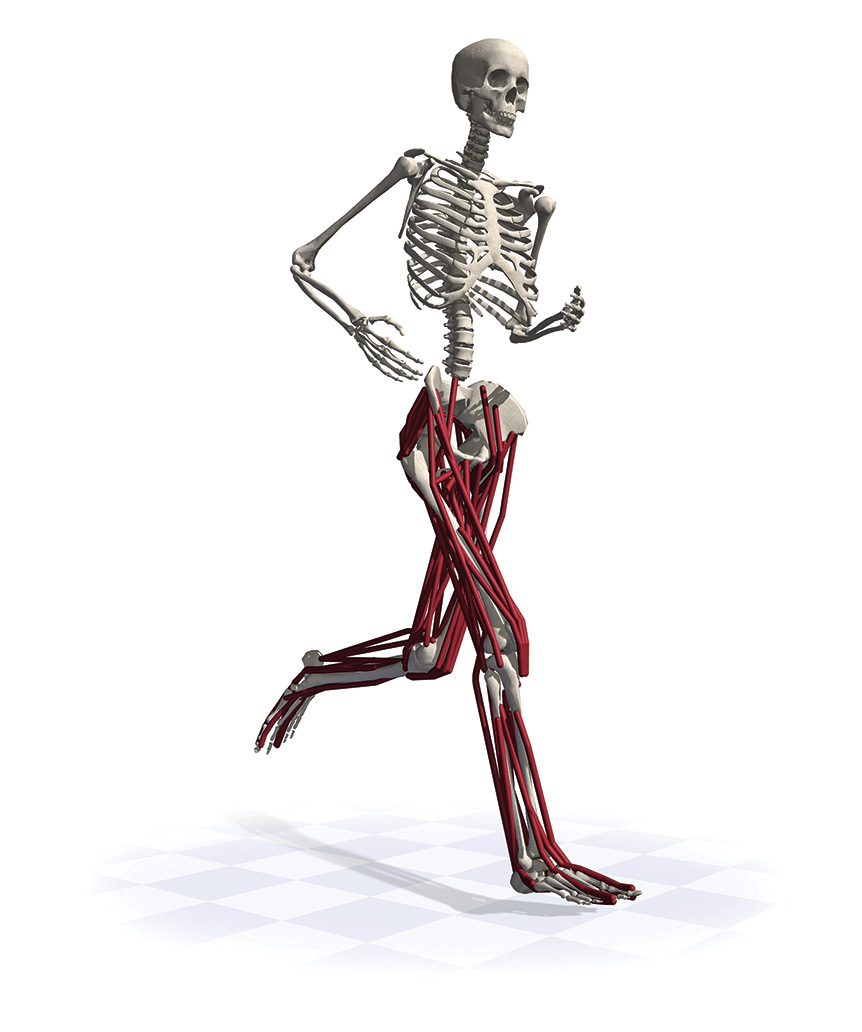
\includegraphics[width=1.0\linewidth]{chap12/12_1}
	\caption{用于生成肌肉驱动的跑步模拟的通用肌肉骨骼模型。
		该模型包含 12 个节段和 29 个自由度,由 86 块下肢肌肉和上身的扭矩执行器驱动\cite{rajagopal2016full} \label{fig:12_1}}
\end{figure}


\section{肌肉对地面反作用力的贡献}

跑步时,重心会因重力和支撑肢肌肉的作用而加速(图~\ref{fig:12_2})。
在支撑初期,\textit{股四头肌}是重心向上和向后加速度的主要贡献者。
在大部分支撑过程中,踝跖屈肌(比目鱼肌和腓肠肌)是重心向上和向前加速度的主要贡献者。
臀大肌在支撑身体重量方面做出了重要贡献。
当然,还有数十块其他肌肉产生力量,影响关节和身体部位的运动。
您可以通过对肌肉驱动的模拟进行详细分析来确定每块肌肉的动作;我们的模拟数据可在 \href{simtk.org}{simtk.org} 上免费获取。


\begin{figure}[!htb]
	\centering
	\includegraphics[width=1.0\linewidth]{chap12/12_2}
	\caption{以 4 米/秒的速度跑步时,臀中肌、股四头肌、比目鱼肌、臀大肌和腓肠肌在站立阶段的活动。
		股四头肌在站立初期最为活跃,此时它们加速重心向上和向后移动;
		腓肠肌和比目鱼肌在整个站立过程中都处于活跃状态,加速重心向上和向前移动。
		臀中肌和臀大肌也对体重支撑做出重要贡献\cite{hamner2010muscle}。 \label{fig:12_2}}
\end{figure}


比目鱼肌是向上和向前重心加速度的最大贡献者,因为它产生的力量巨大,并且只穿过踝关节。
腓肠肌是另一块主要的踝关节跖屈肌,它穿过踝关节和膝关节;
它产生的膝关节屈曲力矩降低了腓肠肌向上加速重心的能力。
跑步时,骨骼排列对重心加速度几乎没有贡献。
慢走时,下肢几乎伸直,骨骼提供被动支撑,但跑步时并非如此。
肌肉力量几乎产生了所有的地面反作用力(图~\ref{fig:12_2}~右上图)。


图~\ref{fig:12_3}~显示了四种速度下跑步时 11 块下肢肌肉的肌电图记录。
这些数据已滤波,以消除高频和低频噪声。
之后,每位受试者的肌电图测量值均被标准化为所有速度下每块肌肉记录的最大值,以获得介于 0 到 1 之间的值。


\begin{figure}[!htb]
	\centering
	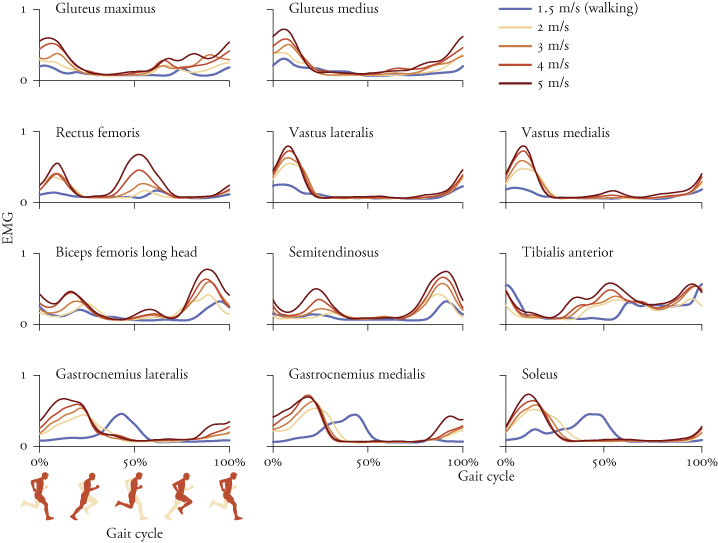
\includegraphics[width=1.0\linewidth]{chap12/12_3}
	\caption{跑步时 11 块肌肉的平均肌电图\cite{arnold2013muscle}。 \label{fig:12_3}}
\end{figure}


我们观察到臀大肌、臀中肌、股直肌、股外侧肌、腓肠肌和比目鱼肌在支撑期的激活程度相对较高。
股直肌在高速奔跑的摆动期开始时激活程度最强;
这块肌肉在髋部和膝部前方交叉,在摆动期开始时加速腿部向前运动。
腘绳肌(股二头肌长头和半腱肌)在摆动期结束时激活程度最强;
这些肌肉在髋部和膝部后方交叉,在摆动期结束时加速腿部向后运动。
胫骨前肌在摆动期最为活跃,用于抬起足部。
随着速度的增加,肌肉活动增加,并且由于支撑期缩短,跖屈肌在步态周期的早期被募集。


正如人们所预料的那样,跑步速度的增加会伴随肌肉激活度的增加,以及由臀大肌、臀中肌、股直肌、股四头肌和腓肠肌产生的向上和前后重心加速度的增加。
通过\textit{肌电图}信号测量的激活度变化如图~\ref{fig:12_3}~所示。
特别要注意的是,当我们从快走转为慢跑时,激活模式会发生巨大变化。
慢跑和快跑之间的区别主要在于幅度,随着速度的增加,股直肌和股二头肌长头等肌肉的活动会急剧增加。
虽然比目鱼肌活动的增加没有那么剧烈,但它却尤为重要。
随着速度的增加,比目鱼肌对向上和向前重心加速度的贡献也会增加。
比目鱼肌在增加飞行​​时间和步幅方面起着关键作用(图~\ref{fig:12_4};表~\ref{tab:12_1}),从而提供了增加跑步速度的机制(公式~\ref{eq:3_1})。

\begin{figure}[!htb]
	\centering
	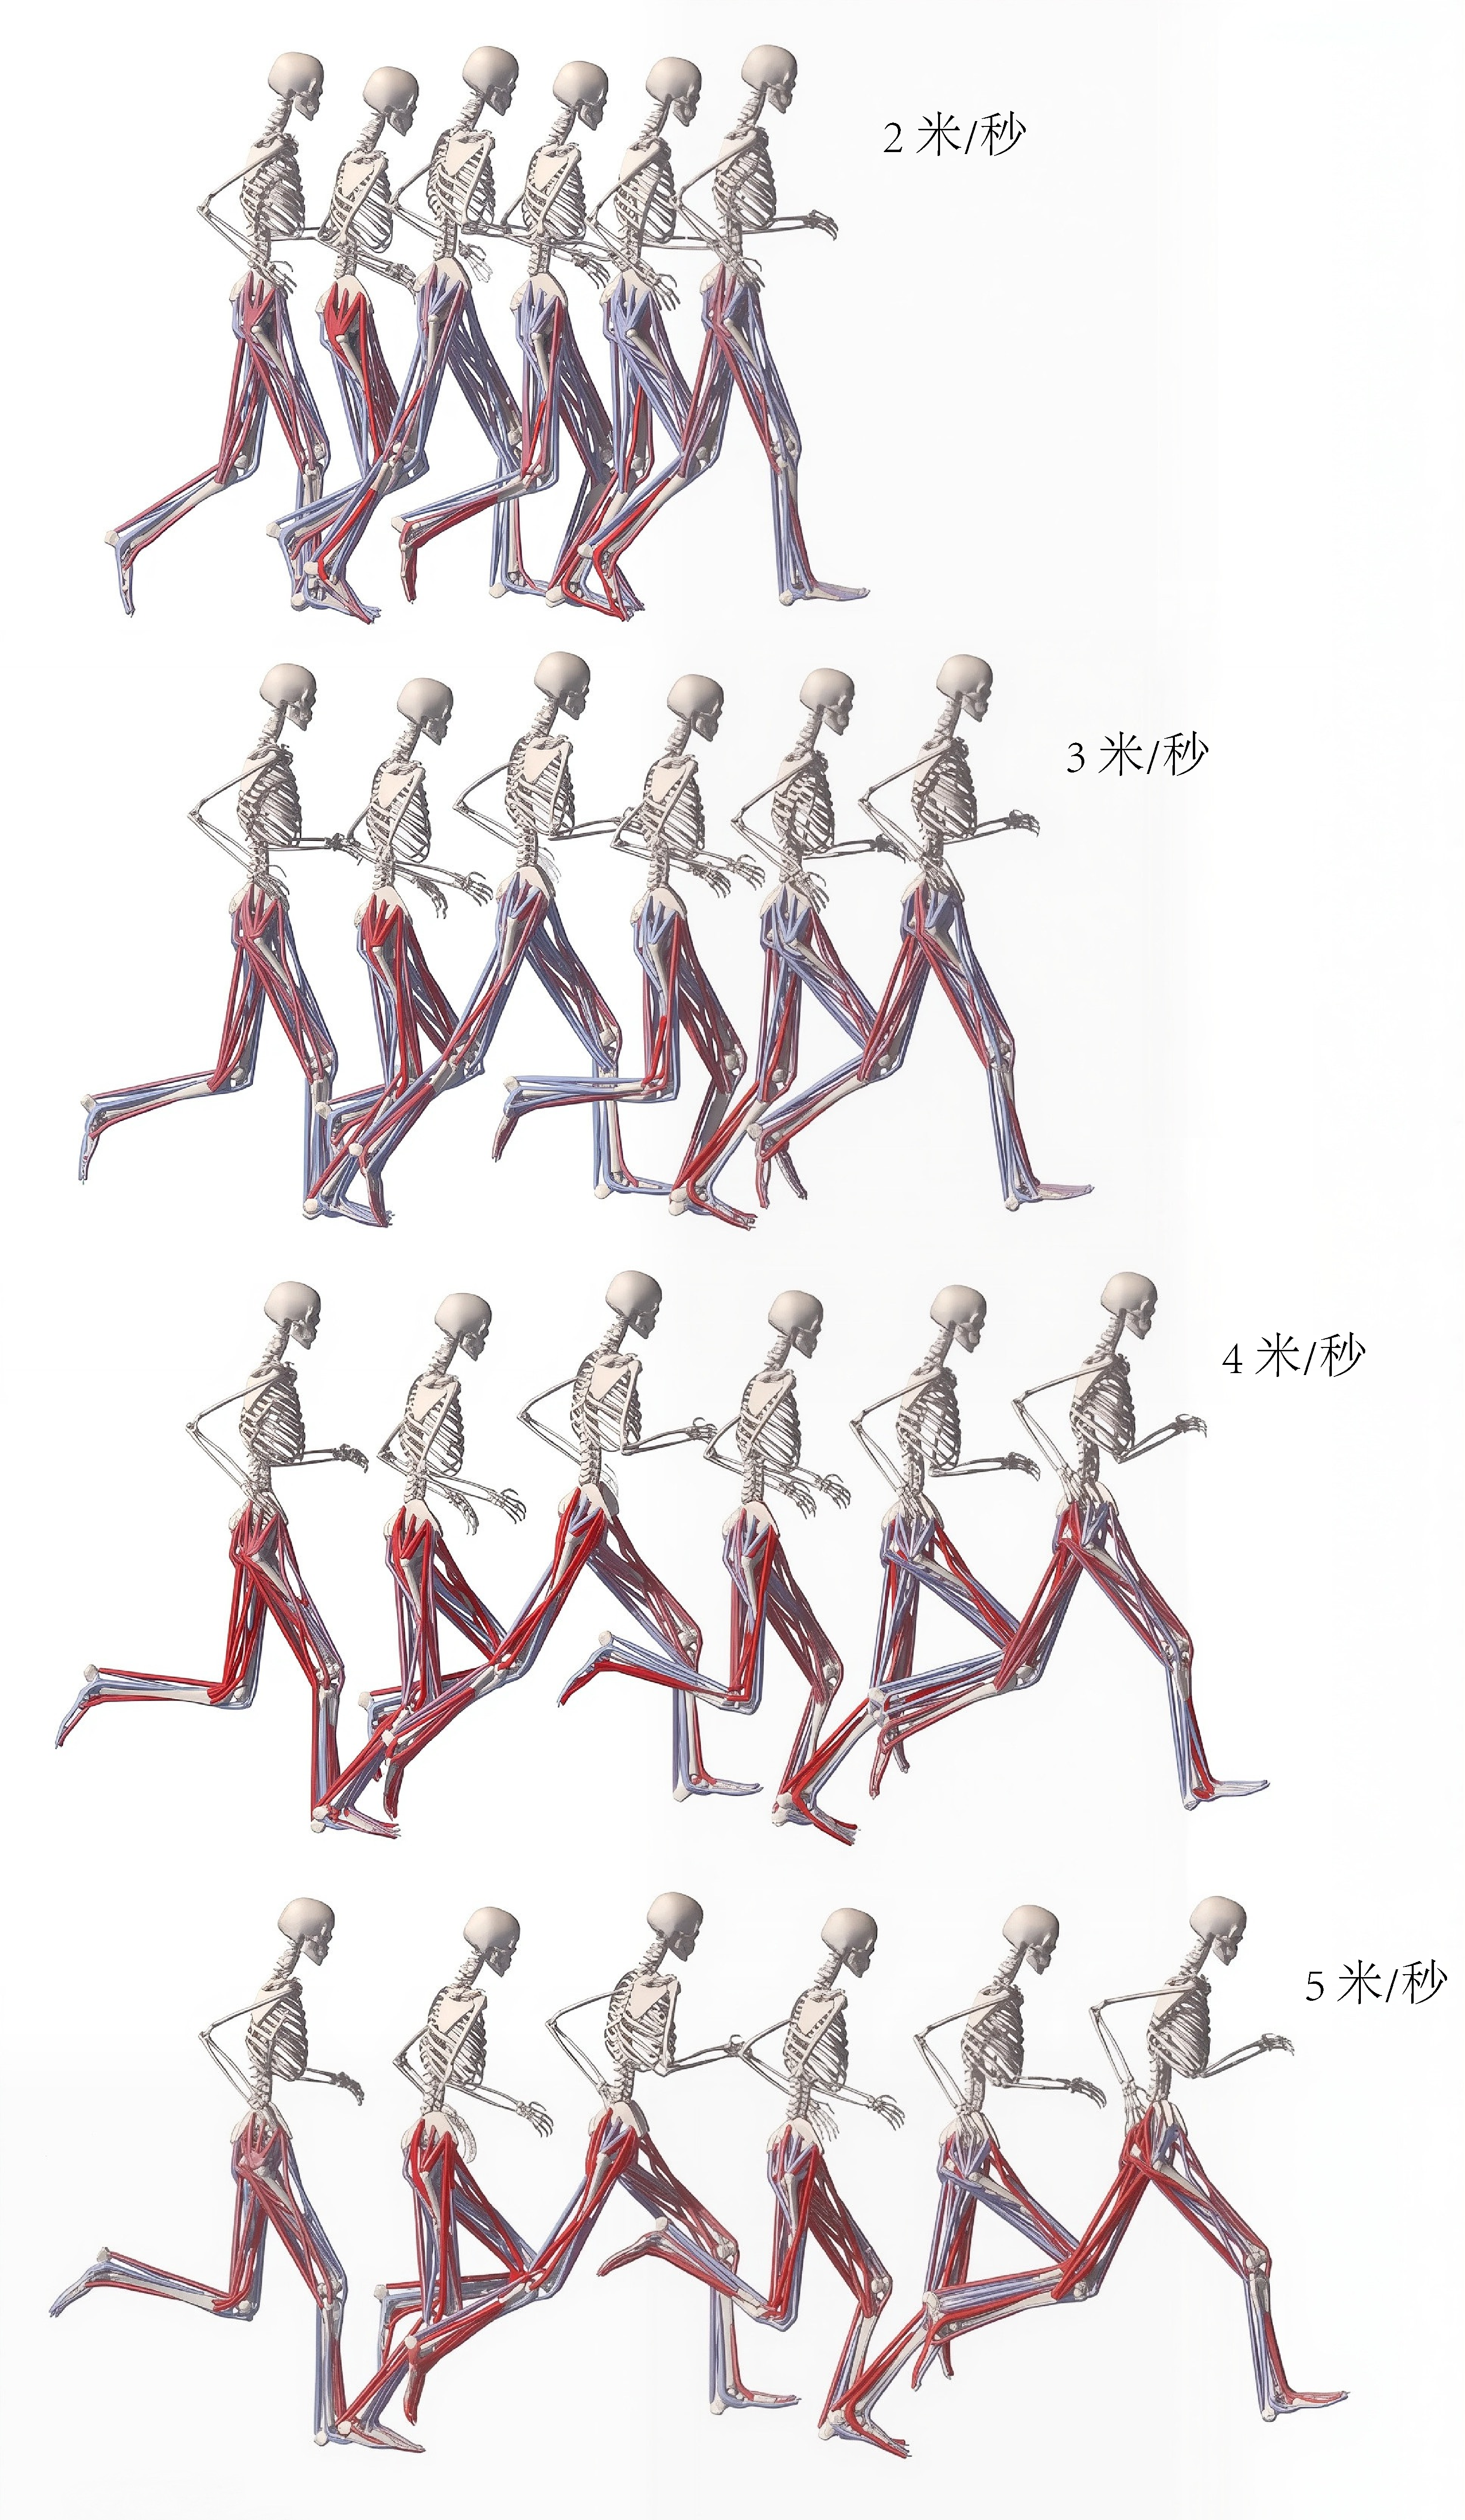
\includegraphics[width=0.8\linewidth]{chap12/12_4}
	\caption{以 4 种速度跑步的代表性受试者的肌肉驱动模拟可视化。
		肌肉颜色表示模拟的激活程度,从无激活(蓝色)到完全激活(红色)\cite{arnold2013muscle}。 \label{fig:12_4}}
\end{figure}


\begin{table}[htbp]
	\caption{跑步参数随速度的变化:脚尖离地时间、步幅、步幅时间和站立时间,取10位受试者的平均值。} \label{tab:12_1} \centering
	\begin{tabular}{ccccc} % l水平左居中,c水平居中
		\toprule
		速度(米/秒)& \makecell{脚趾离地时间\\(步态周期百分比)} & 步幅(米) & 步幅时间(秒) & 站立时间(秒)\\
		\midrule
		2.0 & 47 & 1.5 & 0.75 & 0.34 \\
		3.0 & 40 & 2.1 & 0.71 & 0.29 \\
		4.0 & 38 & 2.7 & 0.67 & 0.26 \\
		5.0 & 38 & 2.7 & 0.67 & 0.26 \\
		7.0$^*$ & 25 & 4.0 & 0.57 & 0.15 \\
		9.0$^*$ & 25 & 4.1 & 0.46 & 0.12 \\
		\bottomrule
	\end{tabular}
\end{table}


当以5米/秒的速度跑步时,比目鱼肌纤维在站立后期缩短的速度是所有肌肉中最快的,这与踝关节跖屈速度加快和站立时间缩短(与低速跑步相比)相吻合。
由于跑步者在更快的跑步速度下会产生更大的向上和向前的重心加速度(即地面反作用力更大),并且比目鱼肌是这些加速度的最大贡献者,因此由于比目鱼肌缩短速度快而导致其力量产生受限,可能会限制跑步者的最高速度。
从积极的角度来说,强壮的比目鱼肌能让跑步者产生增加步幅和跑步速度所需的巨大地面反作用力。


\section{跑步到冲刺的过渡}

我们观察到,在跑步速度高达 5 米/秒时,关节角度的变化会持续到 7 米/秒左右。
通常,最大关节角度会随着速度的增加而持续增大,如图 3.20 所示。
在低于 7 米/秒的速度下,跑步者主要通过产生更大的地面反作用力来提高速度,从而显著增加步幅,而步频仅略有增加(图~\ref{fig:12_5})。
地面反作用力的增加是肌肉“作用力”增加的结果,尤其是在踝跖屈肌中。


\begin{figure}[!htb]
	\centering
	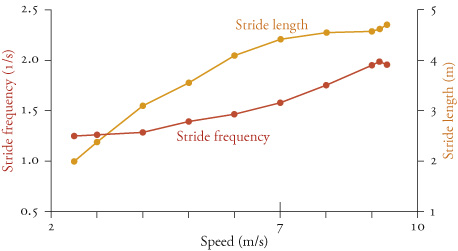
\includegraphics[width=0.75\linewidth]{chap12/12_5}
	\caption{跑步速度的提升主要通过低速时增加步幅、高速时增加步频来实现。
		图中所示数据来自一位代表性受试者\cite{weyand2000faster}。 \label{fig:12_5}}
\end{figure}

肌肉必须产生更大的地面反作用力才能跑得更快,而且必须在更短的时间内产生这些力
(正如杰西$\cdot$欧文斯在本章题词中所言,他通过尽可能减少接触地面的时间来快速奔跑)。
因此,跖屈肌(产生地面反作用力的关键肌肉)会随着跑步速度的增加而缩短得更快。
回想一下,增加肌肉的缩短速度会降低其产生力量的能力(图4.9)。
当速度超过约7米/秒时,踝跖屈肌收缩得非常快,以至于它们无法产生足够的力量来继续增加步幅。


在非常高的奔跑速度下,提高速度的策略并非用更大的力量蹬地,而是转向更频繁地蹬地。
步幅在7米/秒左右时达到最大值;更高的奔跑速度主要通过提高步频来实现。在高速冲刺的摆动阶段,臀部肌肉(主要是髂腰肌、股直肌、臀大肌和腘绳肌)会强力地加速肢体前后运动,从而快速摆动腿部。
因此,最高的奔跑速度是通过在站立时产生较大的地面反作用力(这会产生较大的步幅)以及快速摆动腿部来实现的。
换句话说,我们的最大奔跑速度受限于跖屈肌在高速下产生较大力量的能力,以及臀部和膝盖肌肉摆动腿部的速度。如果你回到图~\ref{fig:3_7},你会注意到,随着跳跃速度的增加,袋鼠的步幅和步频呈现出相似的趋势。


\section{从走转跑过渡过程中的肌肉动作}

人类从步行过渡到跑步的速度约为 2 米/秒,在这个速度下跑步的能量效率更高(图~\ref{fig:3_18})。
运动的大部分代谢成本由肌肉消耗,因此我们预期某些肌肉在从快走过渡到慢跑时会变得更有效率。
事实上,在从步行过渡到跑步的过程中,我们可以在比目鱼肌和腓肠肌及其与跟腱的相互作用中观察到一种有趣的机制。
随着我们走得更快,踝关节跖屈肌的缩短速度会增加,因此在给定的激活水平下,它们产生的力量会更小。
从步行过渡到跑步会通过降低这些肌肉的纤维速度来增强它们产生力量的能力(图~\ref{fig:12_6})。
肌肉驱动的模拟显示,在快走和慢跑之间,腓肠肌外侧肌和比目鱼肌的 $f^\text{V}$(纤维速度对肌肉力量的影响)存在显著差异。
尽管跑步时步速和肌腱单元的缩短速度更快,但从步行到跑步的过渡会降低肌纤维的缩短速度,使腓肠肌外侧肌从向心收缩转为离心收缩,比目鱼肌从向心收缩转为等长收缩。
因此,从步行到跑步的过渡以跖屈肌纤维收缩减慢为特征。这一惊人的结果得到了超声测量\cite{farris2012human}的支持,其原因是跑步时跟腱的拉伸更大,这使得肌肉能够更好地利用更少的能量产生力量。


\begin{figure}[!htb]
	\centering
	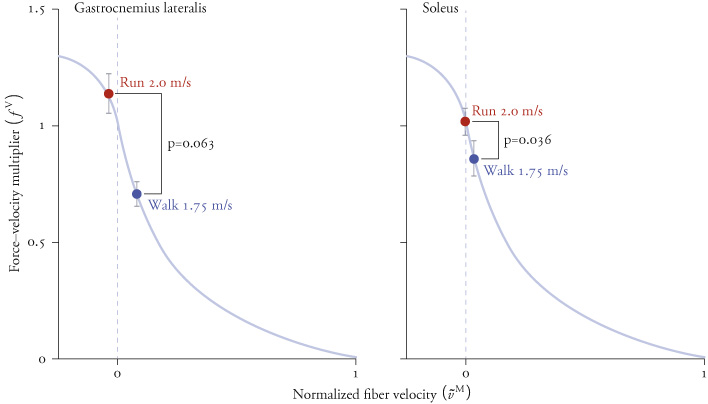
\includegraphics[width=0.9\linewidth]{chap12/12_6}
	\caption{以1.75米/秒(蓝点)行走和以 2.0 米/秒(红点)跑步时,在最大主动力瞬间,力-速度乘数$f^V$的平均值及其标准差($n$ = 5),绘制在力-速度曲线上。
		从步行切换到跑步会降低腓肠肌外侧肌和比目鱼肌的纤维缩短速度,并增加$f^V$ \cite{arnold2013muscle}。 \label{fig:12_6}}
\end{figure}


我们依靠弹性能的储存和释放来执行肌肉和肌腱的伸展和回弹。
由于肌肉通过肌腱附着在骨骼上,肌纤维与肌腱之间的相互作用在决定跑步效率方面起着至关重要的作用。
Lai 等人\cite{lai2014tendon}发现,跟腱的弹性应变能占肌腱正向做功的很大一部分,并且这一比例会随着跑步速度的提高而增加。
正如我们上文所见,跟腱的柔顺性降低了比目鱼肌和腓肠肌纤维在跑步过程中的缩短速度,使它们能够以能够有效发力的长度和速度运作。
柔顺性肌腱还会在跑步过程中储存和释放能量,以延长我们有限的能量预算,类似于电动汽车的再生制动。
在本章的最后,我们将看到一种利用弹性能的储存和释放来降低跑步代谢成本的装置。


\section{手臂和腿部动力学的相互作用}

肌肉驱动模拟表明,在5米/秒或以下的速度下跑步时,手臂对推进力或支撑力的贡献并不显著。
然而,手臂绕过重心的垂直轴的角动量与腿部绕垂直轴的角动量相平衡(即大小相等,方向相反)(图~\ref{fig:12_7})。
跑步速度对手臂和腿部的峰值垂直角动量有显著影响,速度分别从2米/秒时的约1.5千克$\cdot$米$^2$/秒翻倍至5米/秒时的3.0千克$\cdot$米$^2$/秒。


\begin{figure}[!htb]
	\centering
	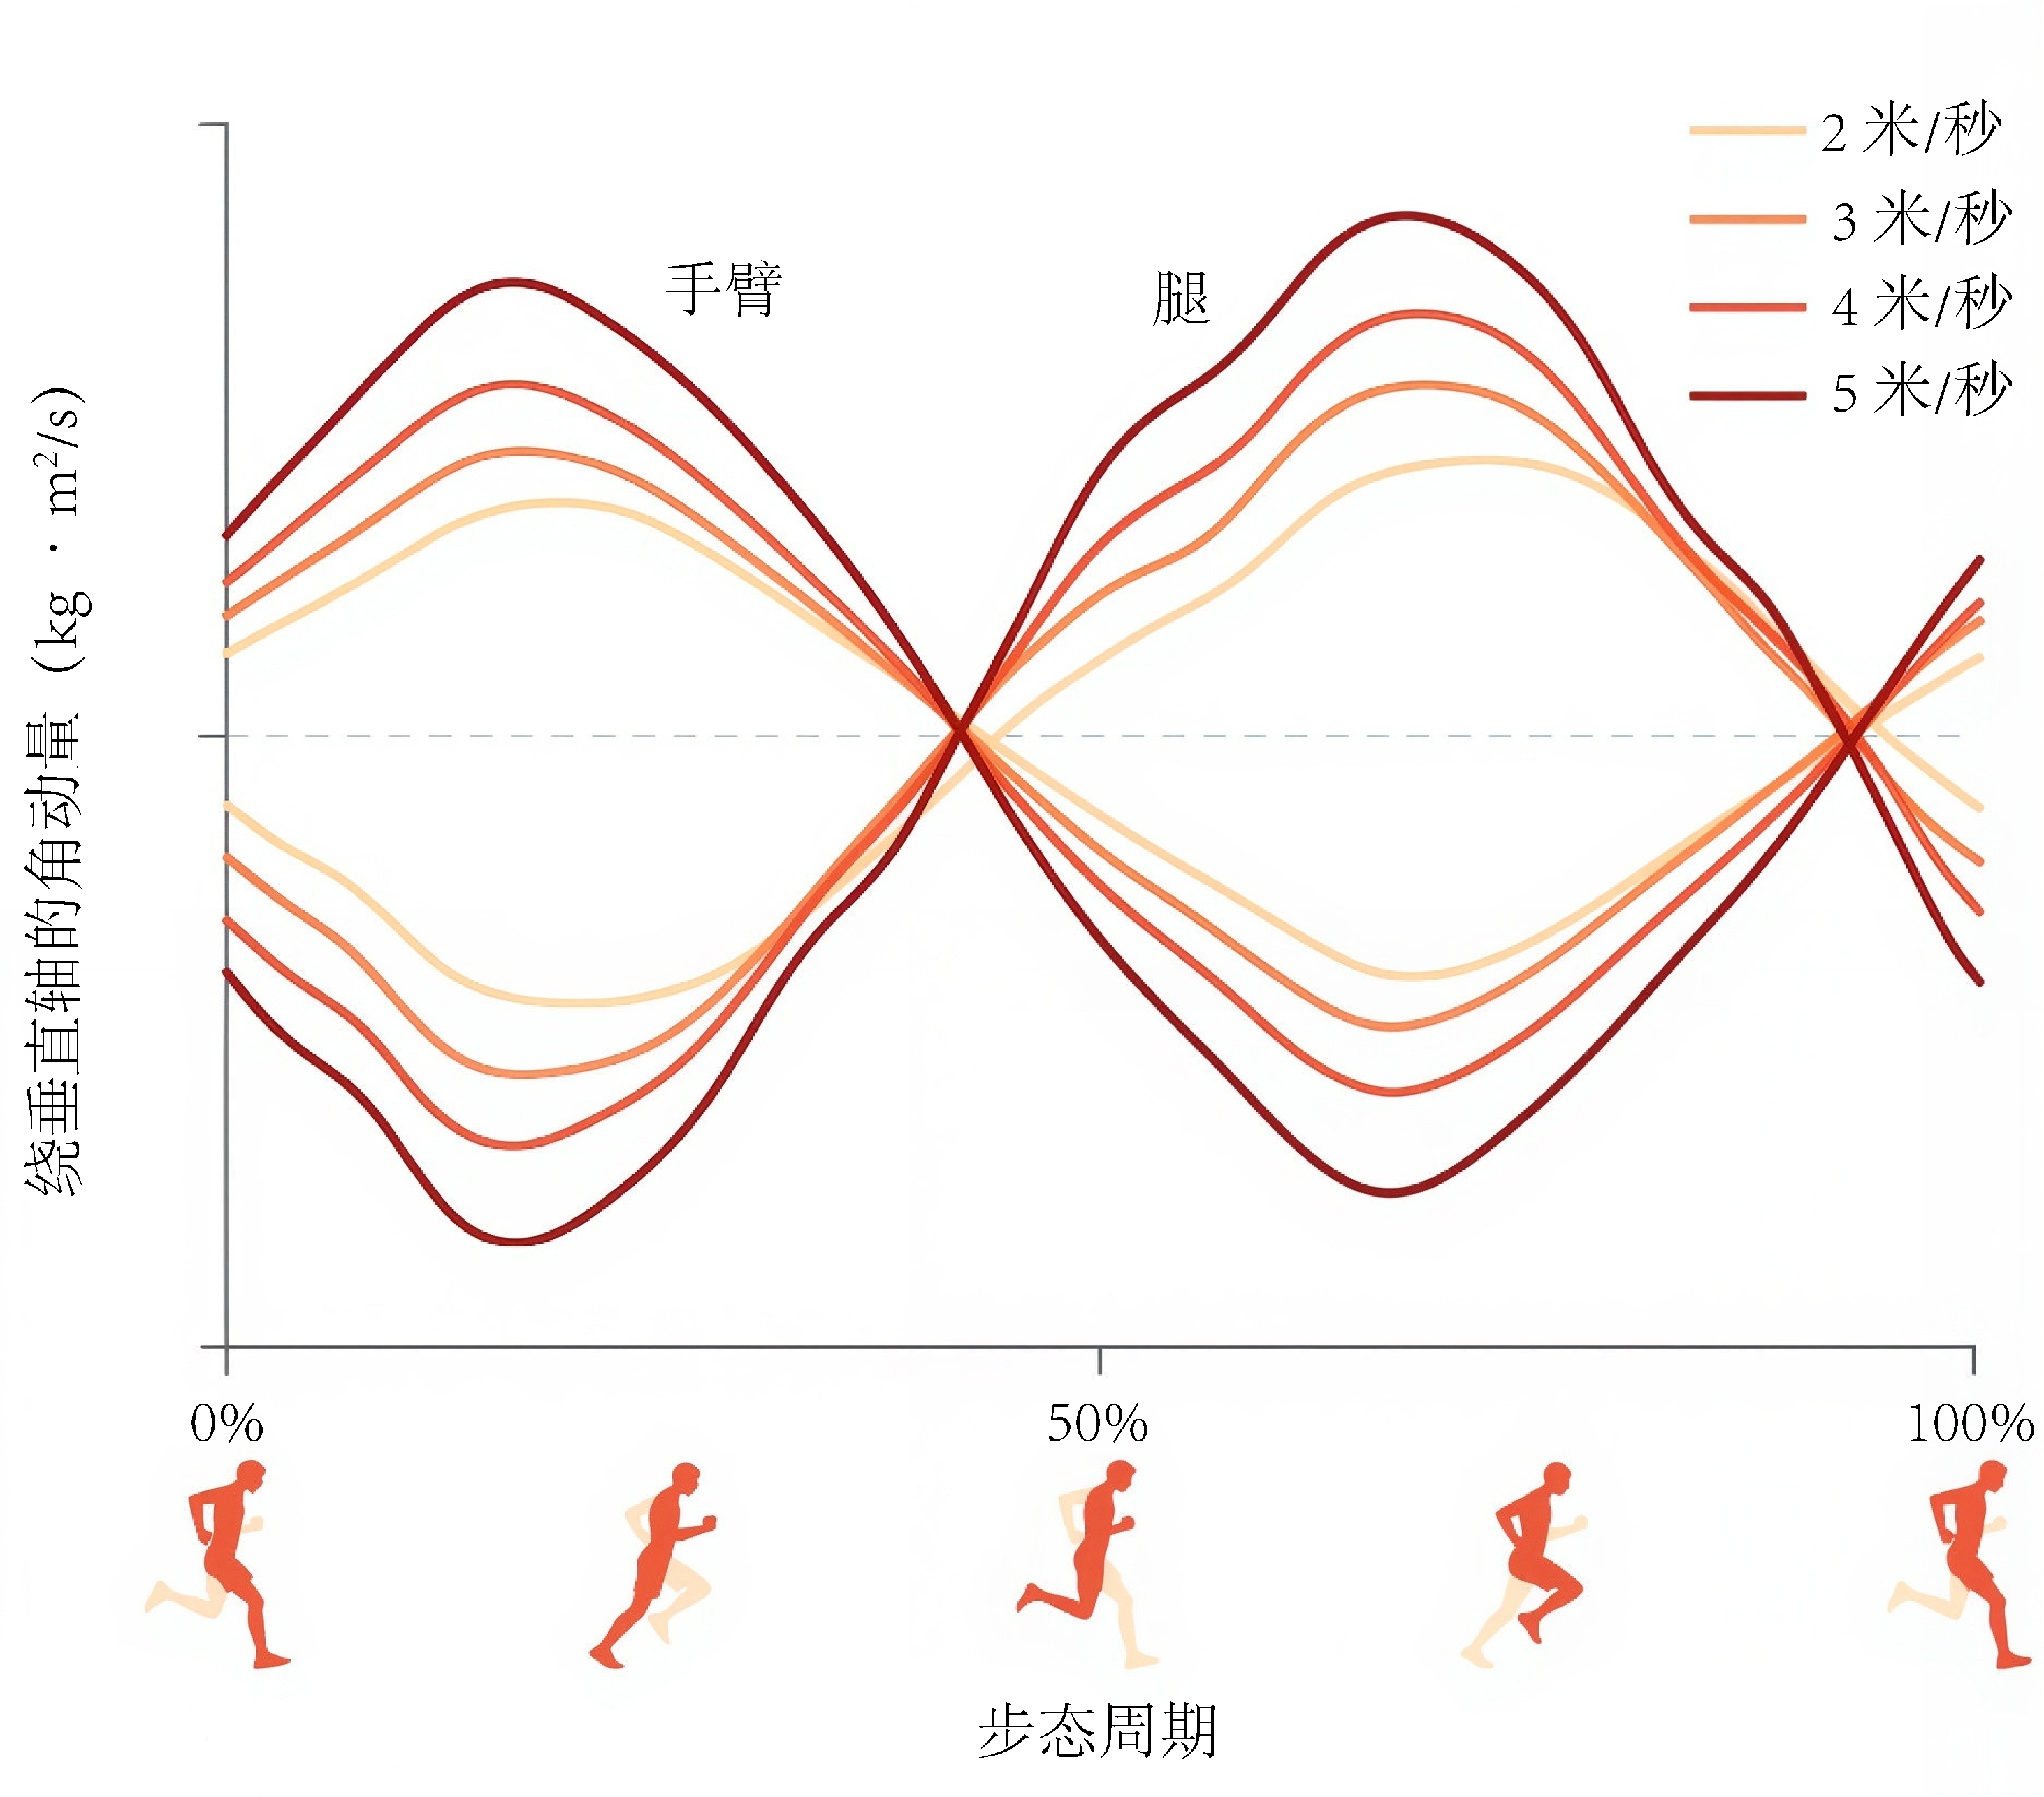
\includegraphics[width=0.75\linewidth]{chap12/12_7}
	\caption{跑步时手臂和腿部绕穿过身体重心的垂直轴的反向角动量,取 10 名受试者的平均值\cite{hamner2013muscle}。 \label{fig:12_7}}
\end{figure}


\section{跑步时摆动双腿}

21 世纪初,Jesse Modica 和 Rodger Kram 试图了解肌肉在跑步过程中腿部摆动中的作用以及在此过程中消耗的代谢能量。
他们记录了关键肌肉的肌电图,并测量了中速跑步机跑步时的全身代谢成本。
仅根据肌电图计时,人们可以推测股直肌和腿筋负责启动和阻止腿部摆动。
为了验证这一假设,Modica 和 Kram 构建了一个巧妙的装置,仅在摆动阶段的第一部分向每只脚施加向前的力(图~\ref{fig:12_8})。
在辅助跑步过程中,他们观察到摆动前半段股直肌活动显着减少,但腓肠肌或比目鱼肌肌电图没有减少,这表明股直肌在自然(无辅助)跑步过程中的腿部摆动中起着重要作用这项研究及后续研究表明,腿部摆动约占中速跑步时能量消耗的10\%至20\%。
其余能量则用于支撑身体重量并推动身体向前。

\begin{figure}[!htb]
	\centering
	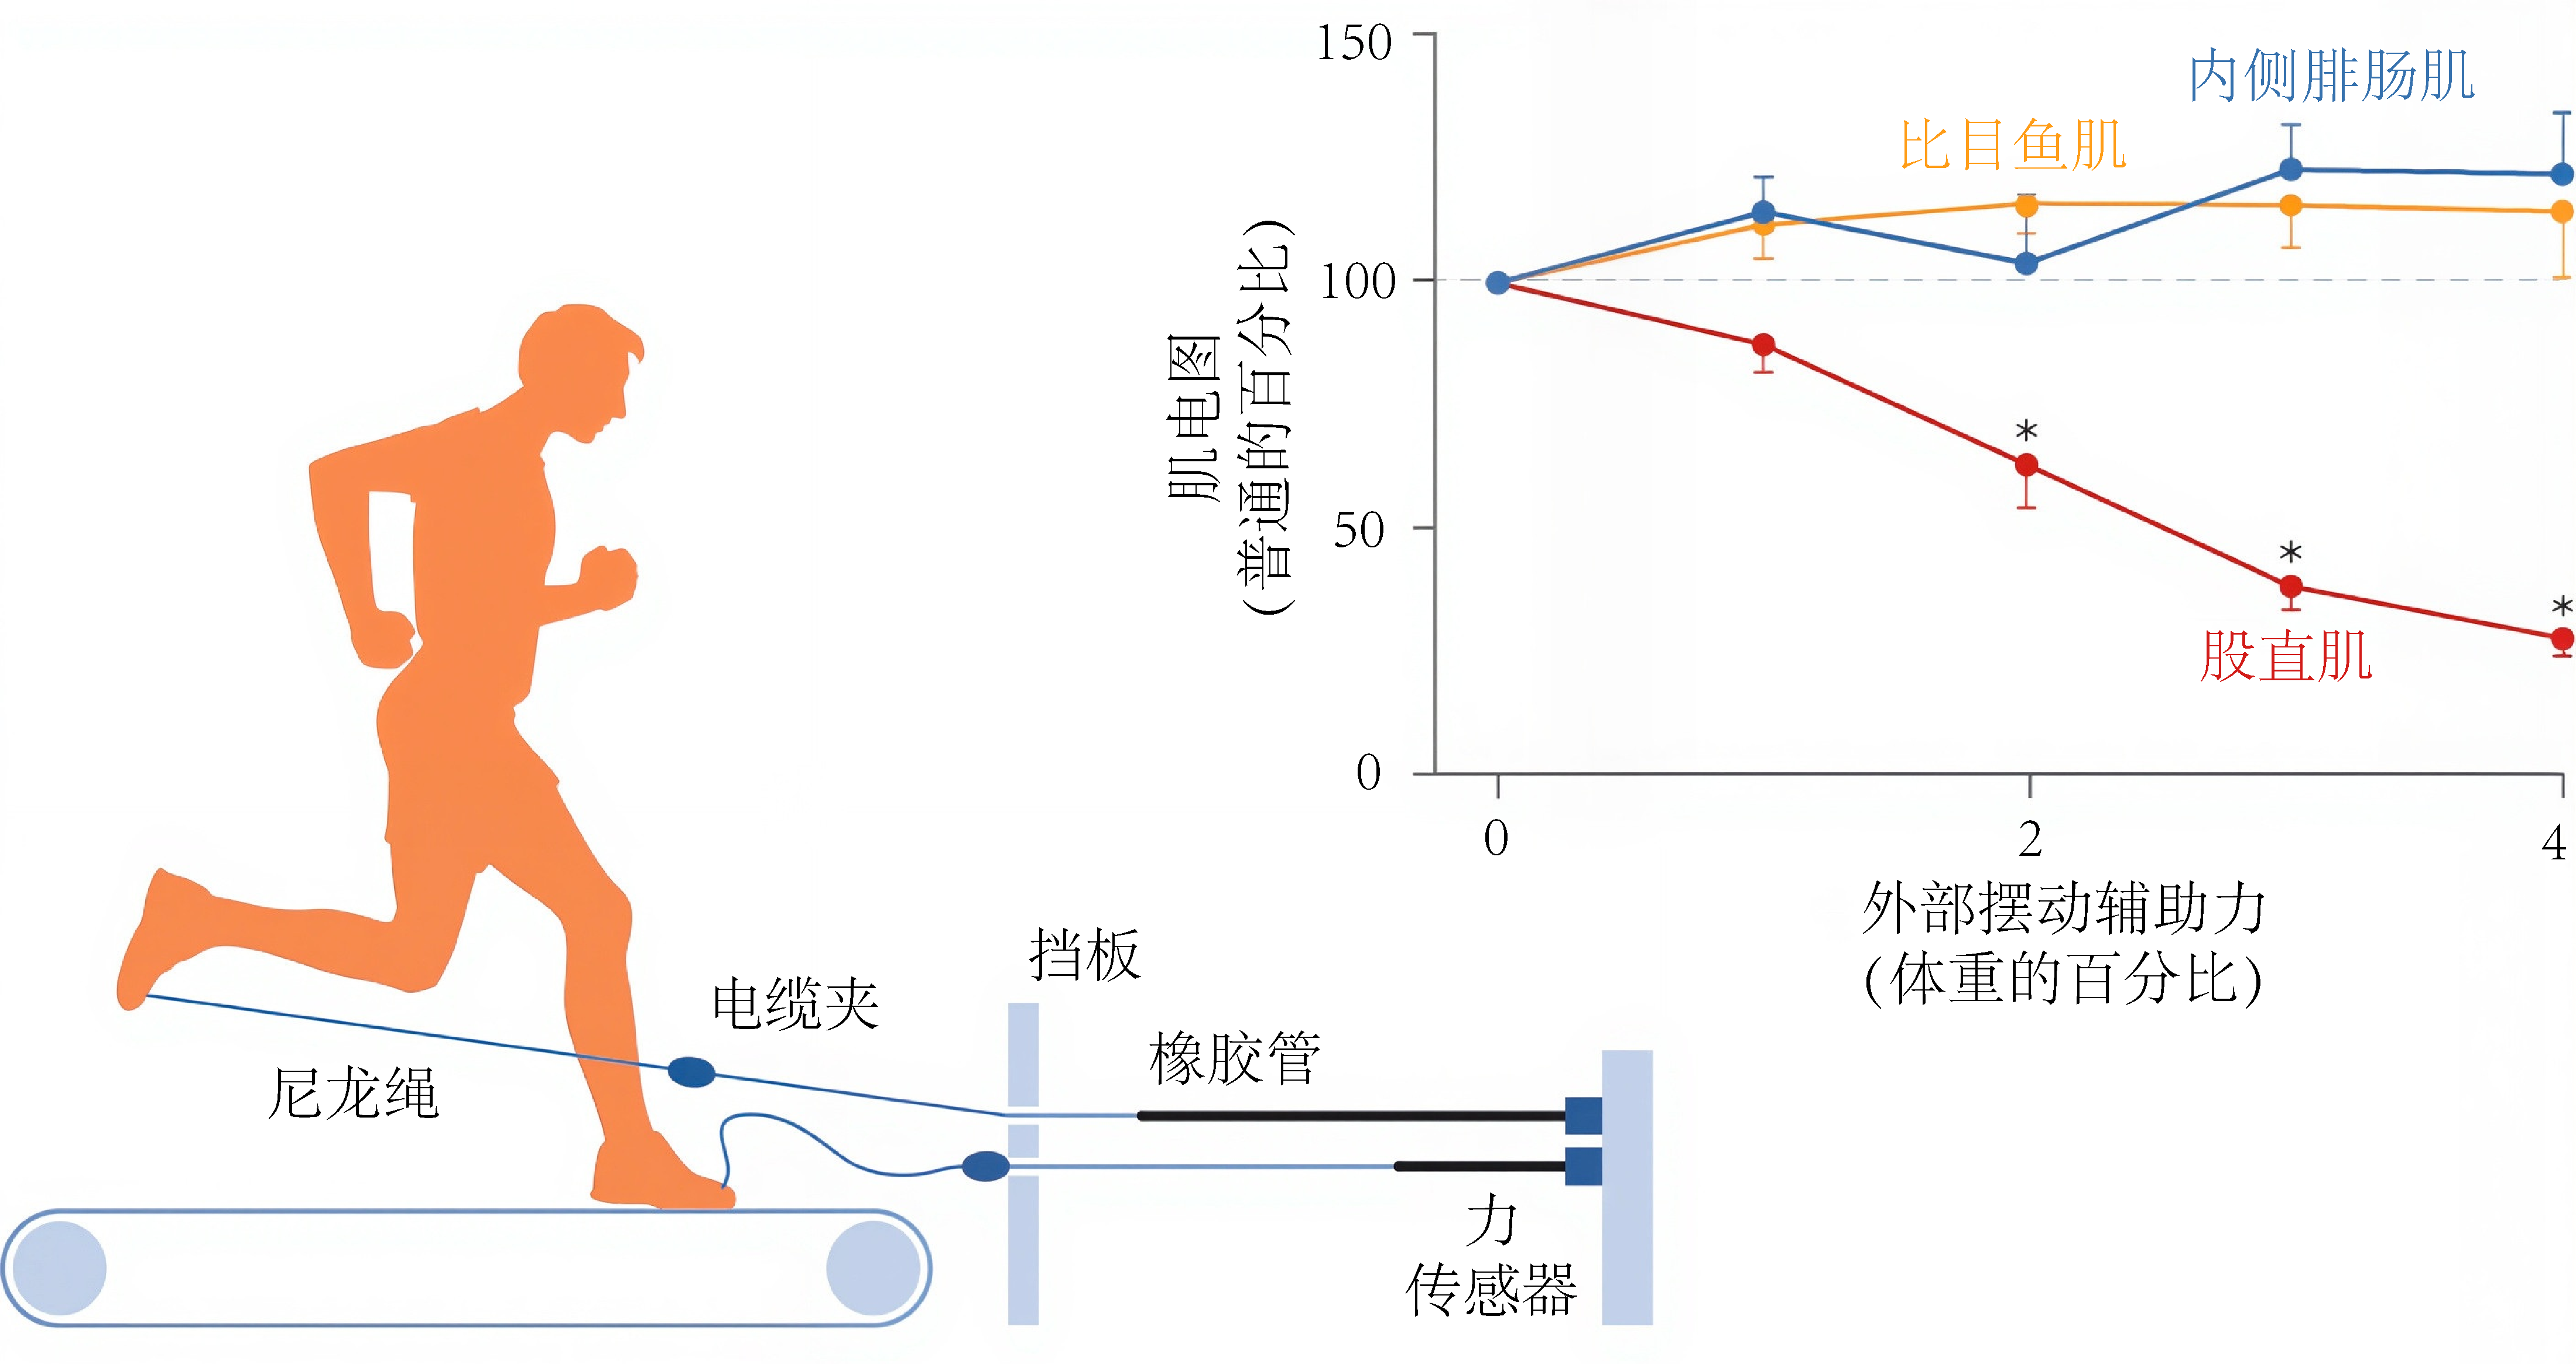
\includegraphics[width=1.0\linewidth]{chap12/12_8}
	\caption{跑步机跑步时摆动辅助机制及其对肌电图的影响。
		左图:站立时,橡胶管随着足部向后移动而拉伸,在摆动开始时对足部施加前向力,并在电缆夹接触止动板时松弛。
		右图:跑步过程中,随着摆动辅助的增加,肌电图幅值的变化,取无辅助跑步时各肌肉活跃时段的平均值($n$ = 10,平均值±标准误差;*p < 0.0001)\cite{modica2005metabolic}。 \label{fig:12_8}}
\end{figure}



\section{脚步模式}

在第~\ref{chap:chap11}~章中,我们了解到踝关节跖屈肌严重紧张的人会采用“足尖行走”的姿势。
肌肉健康的人很少会采用足尖行走(尽管偶尔会在短距离内偷袭他人)。
相比之下,许多健康的跑步者天生前脚掌着地,他们落地时脚掌前部而不是脚后跟(图~\ref{fig:12_9})。
跑步教练们争论的是前脚掌着地还是后脚掌着地更好。
绝大多数长跑运动员都是后脚掌着地,但这两种着地方式都没有被证明更有效。


\begin{figure}[!htb]
	\centering
	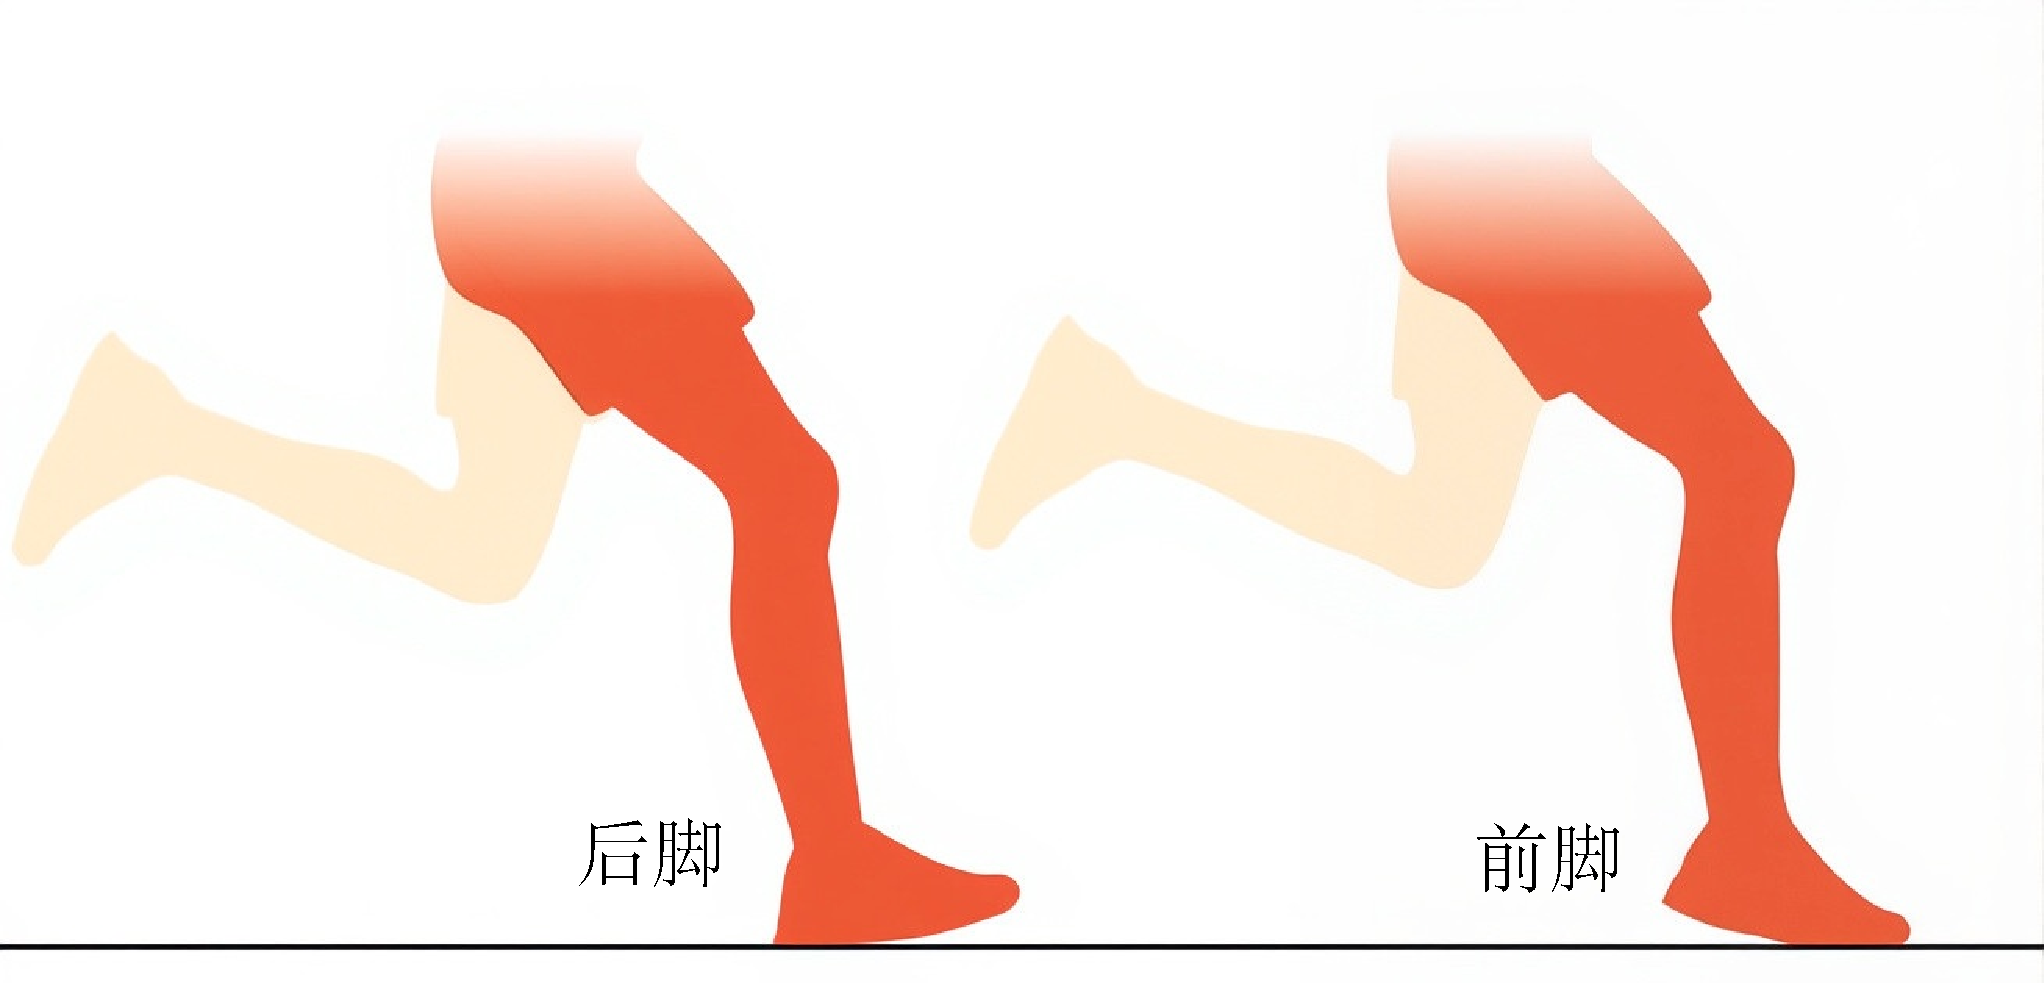
\includegraphics[width=0.5\linewidth]{chap12/12_9}
	\caption{跑步时的脚步模式。 \label{fig:12_9}}
\end{figure}


这些脚部着地模式的运动学和动力学明显不同。
我们在第~\ref{chap:chap3}~章中看到,前脚掌着地的跑步者所受的垂直地面反作用力比后脚掌着地的跑步者上升得更缓慢(比较图3.2和3.3),这让人们相信前脚掌着地可能有助于预防骨骼应力性骨折。
然而,前脚掌着地时跟腱的应变率更高\cite{lyght2016effects},这表明前脚掌着地比后脚掌着地更容易造成肌腱损伤。
事实上,习惯性后脚掌着地的跑步者报告称,在转换为前脚掌着地时,小腿肌肉会感到酸痛,这表明跖屈肌和跟腱在两种跑步方式中可能承受不同的负荷。


为了检验前脚掌和后脚掌着地时跖屈肌腱力学的差异,我实验室的 Jenny Yong 等人使用 16 名健康跑步者的数据生成了模拟数据。
所有跑步者都是习惯性后脚掌着地的跑步者,其中一组模拟数据是在他们以自然速度和习惯性后脚掌着地步态跑步时收集的数据生成的。
然后,跑步者接受了一项训练方案,学习采用前脚掌着地的模式。
第二组模拟数据是在跑步时前脚掌着地时收集的数据生成的。
我们测量了运动学数据(用于规定肌肉驱动模型的关节角度)和\textit{肌电图}数据,将其处理后作为激励应用于模拟的肌肉。
这些模拟数据用于计算肌肉激活度、纤维长度、纤维速度以及每块肌肉产生主动力的能力(图~\ref{fig:12_10})。

\begin{figure}[!htb]
	\centering
	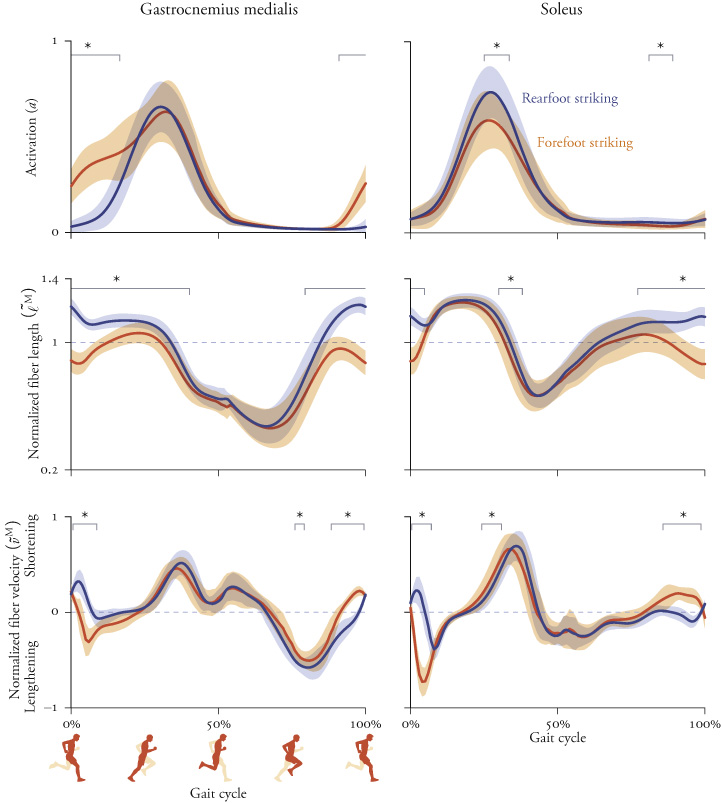
\includegraphics[width=1.0\linewidth]{chap12/12_10}
	\caption{模拟以2.94 ± 0.30米/秒的速度跑步,同时后脚掌和前脚掌着地时,跖屈肌的肌肉激活度和纤维动力学(n = 16,平均值±1个标准差;*p < 0.05)\cite{yong2020foot}。 \label{fig:12_10}}
\end{figure}


我们的模拟显示,足部着地模式对腓肠肌和比目鱼肌的影响有所不同。
前脚掌着地时,腓肠肌在站立初期的激活程度较高,导致腓肠肌纤维和跟腱相应部分的力量更大。
相比之下,前脚掌着地时,比目鱼肌在蹬地时(约占步态周期的25\%)的激活程度较低。


足部着地模式对腓肠肌和比目鱼肌的影响也存在相似之处。
在前脚着地时,从摆动后期到站立初期,这两块肌肉的纤维都较短,并且纤维速度在摆动后期较低,但在站立初期较高。
在站立初期的大部分时间里,跖屈肌纤维在后脚着地时缩短,而在前脚着地时延长。


有趣的是,尽管前脚掌着地时看起来富有弹性,但这种着地模式并不影响腓肠肌腱储存的能量(表面差异在统计学上并不显著),而且比目鱼肌腱在前脚掌着地时储存的能量实际上更少(图~\ref{fig:12_11},上)。
前脚掌和后脚掌着地时,跟腱储存的总能量并无差异;
然而,不同着地模式的能量储存和释放时间却截然不同(图~\ref{fig:12_11},下)。

\begin{figure}[!htb]
	\centering
	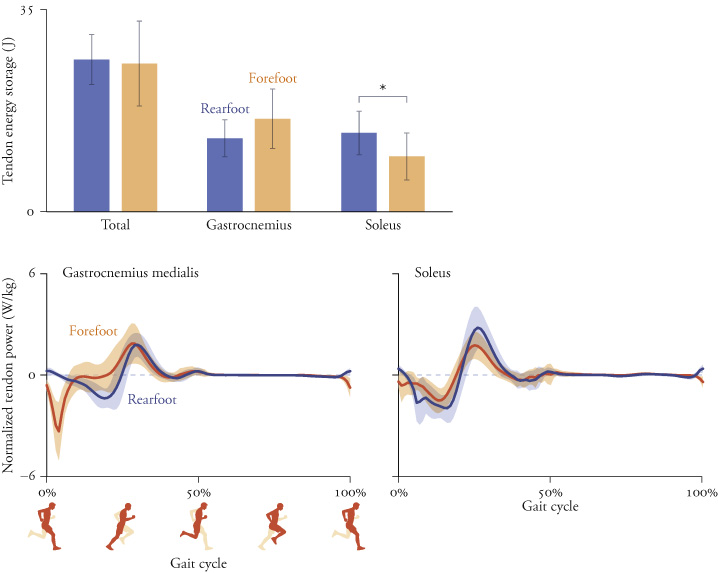
\includegraphics[width=1.0\linewidth]{chap12/12_11}
	\caption{模拟跑步时后足和前足着地时跖屈肌腱的弹性能量(上)和功率(下)($n = 16$,平均值±1个标准差;*p < 0.05)\cite{yong2020foot}。\label{fig:12_11}}
\end{figure}


前脚掌着地会提高腓肠肌纤维在站立初期(此时肌肉正在产生巨大的力量并被拉伸)吸收能量的速率。
肌肉在拉伸过程中产生巨大的力量时容易受伤,这或许可以解释为什么一些后脚掌着地的跑者在尝试转换为前脚掌着地时会报告小腿肌肉酸痛。
我建议那些计划转换为前脚掌着地的跑者在转换之前,先进行渐进式离心腓肠肌强化训练,以避免肌肉受伤。


\section{设备辅助跑步}

辅助设备可以与我们的肌肉骨骼系统互动,从而恢复活动能力并提升运动表现。这项技术的众多潜在应用之一是降低跑步的代谢成本。
Thomas Uchida 使用肌肉驱动的跑步模拟来探索辅助设备的生物力学和能量效应\cite{uchida2016simulating}。
这些模拟设备没有质量,能够瞬间、精准地将巨大的扭矩直接传递到骨骼上。
这些模拟使得我们能够在不构建原型的情况下比较辅助设备,并且不受诸如力传递不完美等混杂因素的影响。
Uchida 使用肌肉驱动的模拟,模拟 10 名运动员在跑步机上以 2 米/秒和 5 米/秒的速度跑步。
他使用理想的辅助设备增强了图~\ref{fig:12_1}~所示的肌肉骨骼模型,这些辅助设备可在髋部、膝盖和脚踝处提供屈曲和伸展力矩,然后确定了使模拟肌肉激活平方和最小化的辅助模式。
使用肌肉纤维所消耗的能量作为其兴奋、激活、长度和速度的函数的模型来估算有辅助和无辅助跑步的代谢成本\cite{umberger2003model,uchida2016simulating}。


模拟结果预测,在两种跑步速度下,所有辅助场景下的代谢成本均会大幅降低(图~\ref{fig:12_12})。
以2米/秒的速度跑步时,踝部、膝盖和臀部装置的效果相同,平均代谢功率降低 1.5 瓦/千克,约为无辅助跑步时代谢功率的四分之一。
然而,以 5 米/秒的速度跑步时,臀部装置降低代谢成本的效果显著优于踝部或膝盖装置(p < 0.002)。
这一结果表明,辅助装置应根据用户的跑步速度,随着速度的增加,将装置功率从踝部重新分配到臀部。

\begin{figure}[!htb]
	\centering
	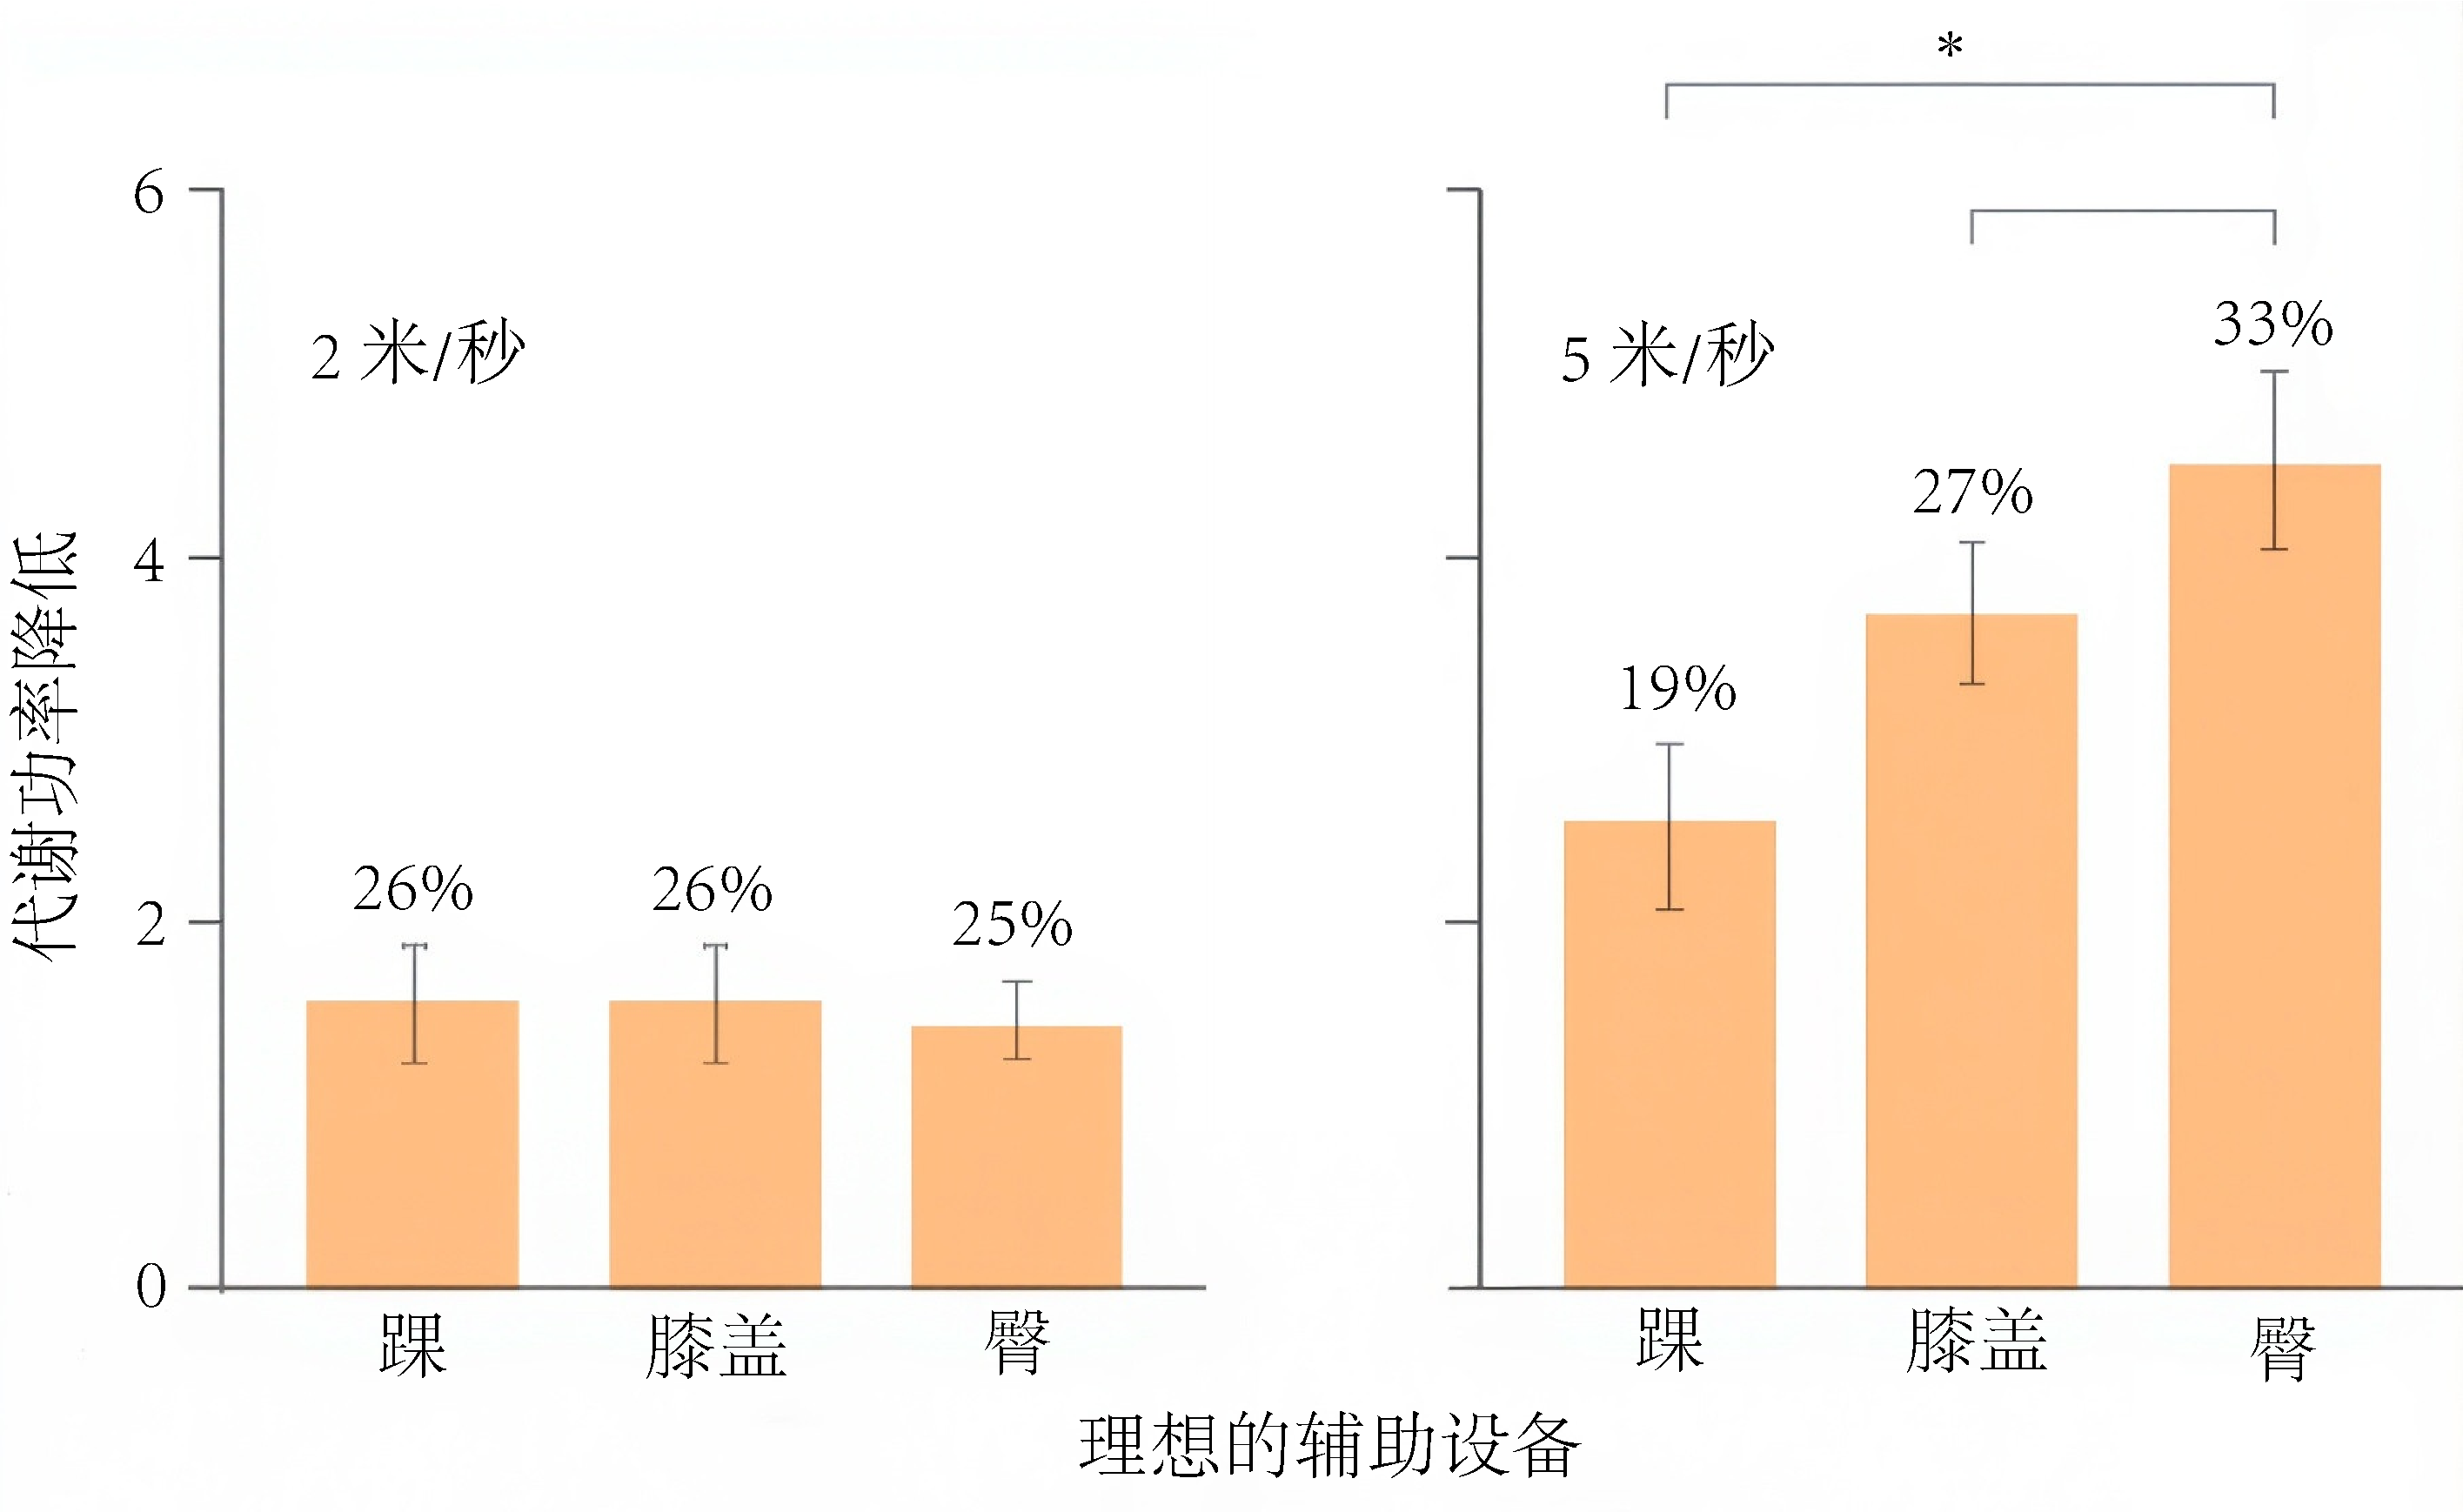
\includegraphics[width=0.75\linewidth]{chap12/12_12}
	\caption{肌肉骨骼模型在理想屈伸辅助装置辅助下,下肢肌肉能量消耗减少(阴影柱代表平均值;直线代表标准差;$n = 10$;*p < 0.002)。
		平均功率以受试者体重(W/kg)标准化,并计算各速度下无辅助跑步的能耗百分比\cite{uchida2016simulating}。 \label{fig:12_12}}
\end{figure}


图~\ref{fig:12_13}~显示了以 5 米/秒的速度跑步时,每种辅助设备对 9 块肌肉协调性的影响。
在辅助关节处,肌肉激活度通常会降低;
然而,在非辅助关节处,肌肉激活度也会降低;
而当增加辅助时,一些肌肉的激活度会增加。
在踝关节处增加辅助后,比目鱼肌和胫骨前肌的激活度在整个步态周期中急剧下降,因为这些肌肉只产生踝关节力矩。
腓肠肌的激活度在站立时仅部分降低;
虽然它不再负责产生踝关节跖屈力矩,但它仍然被调动来产生(非辅助)膝关节的屈曲力矩。
原始腓肠肌激活度的剩余部分大致反映了其在站立时产生膝关节屈曲力矩的活性。
在膝关节处增加辅助后,我们观察到股直肌在早期摆动时的激活度增加,以利用其纤维延长后相对较高的产力能力。
股直肌产生的髋屈曲力矩增大,导致腰大肌活动减少。
当髋部增加支撑时,观察到肌肉活动发生复杂的变化。


\begin{figure}[!htb]
	\centering
	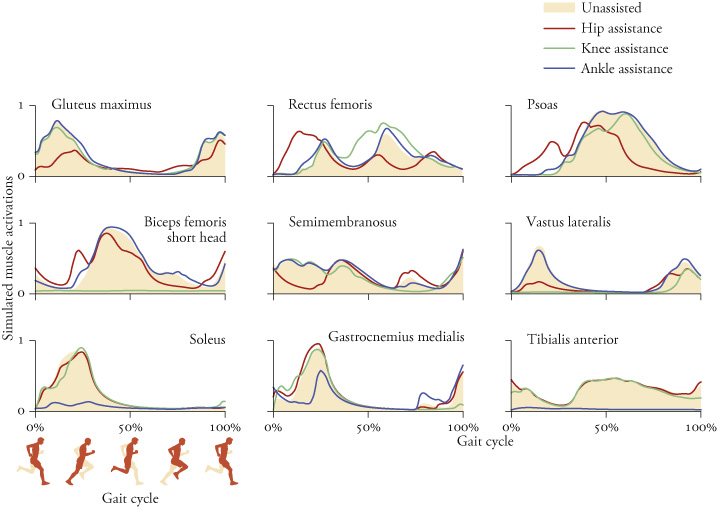
\includegraphics[width=1.0\linewidth]{chap12/12_13}
	\caption{在使用理想屈伸辅助设备模拟以 5 米/秒速度跑步时,9 块代表性下肢肌肉的激活情况(平均值;$n = 10$)\cite{uchida2016simulating}。 \label{fig:12_13}}
\end{figure}


对辅助的补偿可能很复杂。
像这样的肌肉驱动模拟是对实验的重要补充,因为它们为观察到的效果提供了生物力学解释,并为未来的实验研究提出了假设。
我们的模拟证明了在设计辅助策略时考虑整个下肢肌肉协调的重要性。
正如我们在第~\ref{chap:chap11}~章中看到的设备辅助行走一样,最佳设备扭矩曲线通常与无辅助跑步时肌肉产生的相应净关节力矩不同。
这一发现得到了哈佛大学康纳$\cdot$沃尔什 (Connor Walsh) 领导的团队的证实,他们利用我们的研究结果来确定他们的辅助设备应施加什么样的髋部伸展扭矩来降低跑步时的代谢成本(图~\ref{fig:12_14})。
当应用无辅助时肌肉产生的净髋部伸展力矩的缩放版本时,他们的设备仅将净代谢功耗降低了 0.11 W/kg。
根据我们的模拟结果得出的扭矩曲线的效率是其 4 倍。


\begin{figure}[!htb]
	\centering
	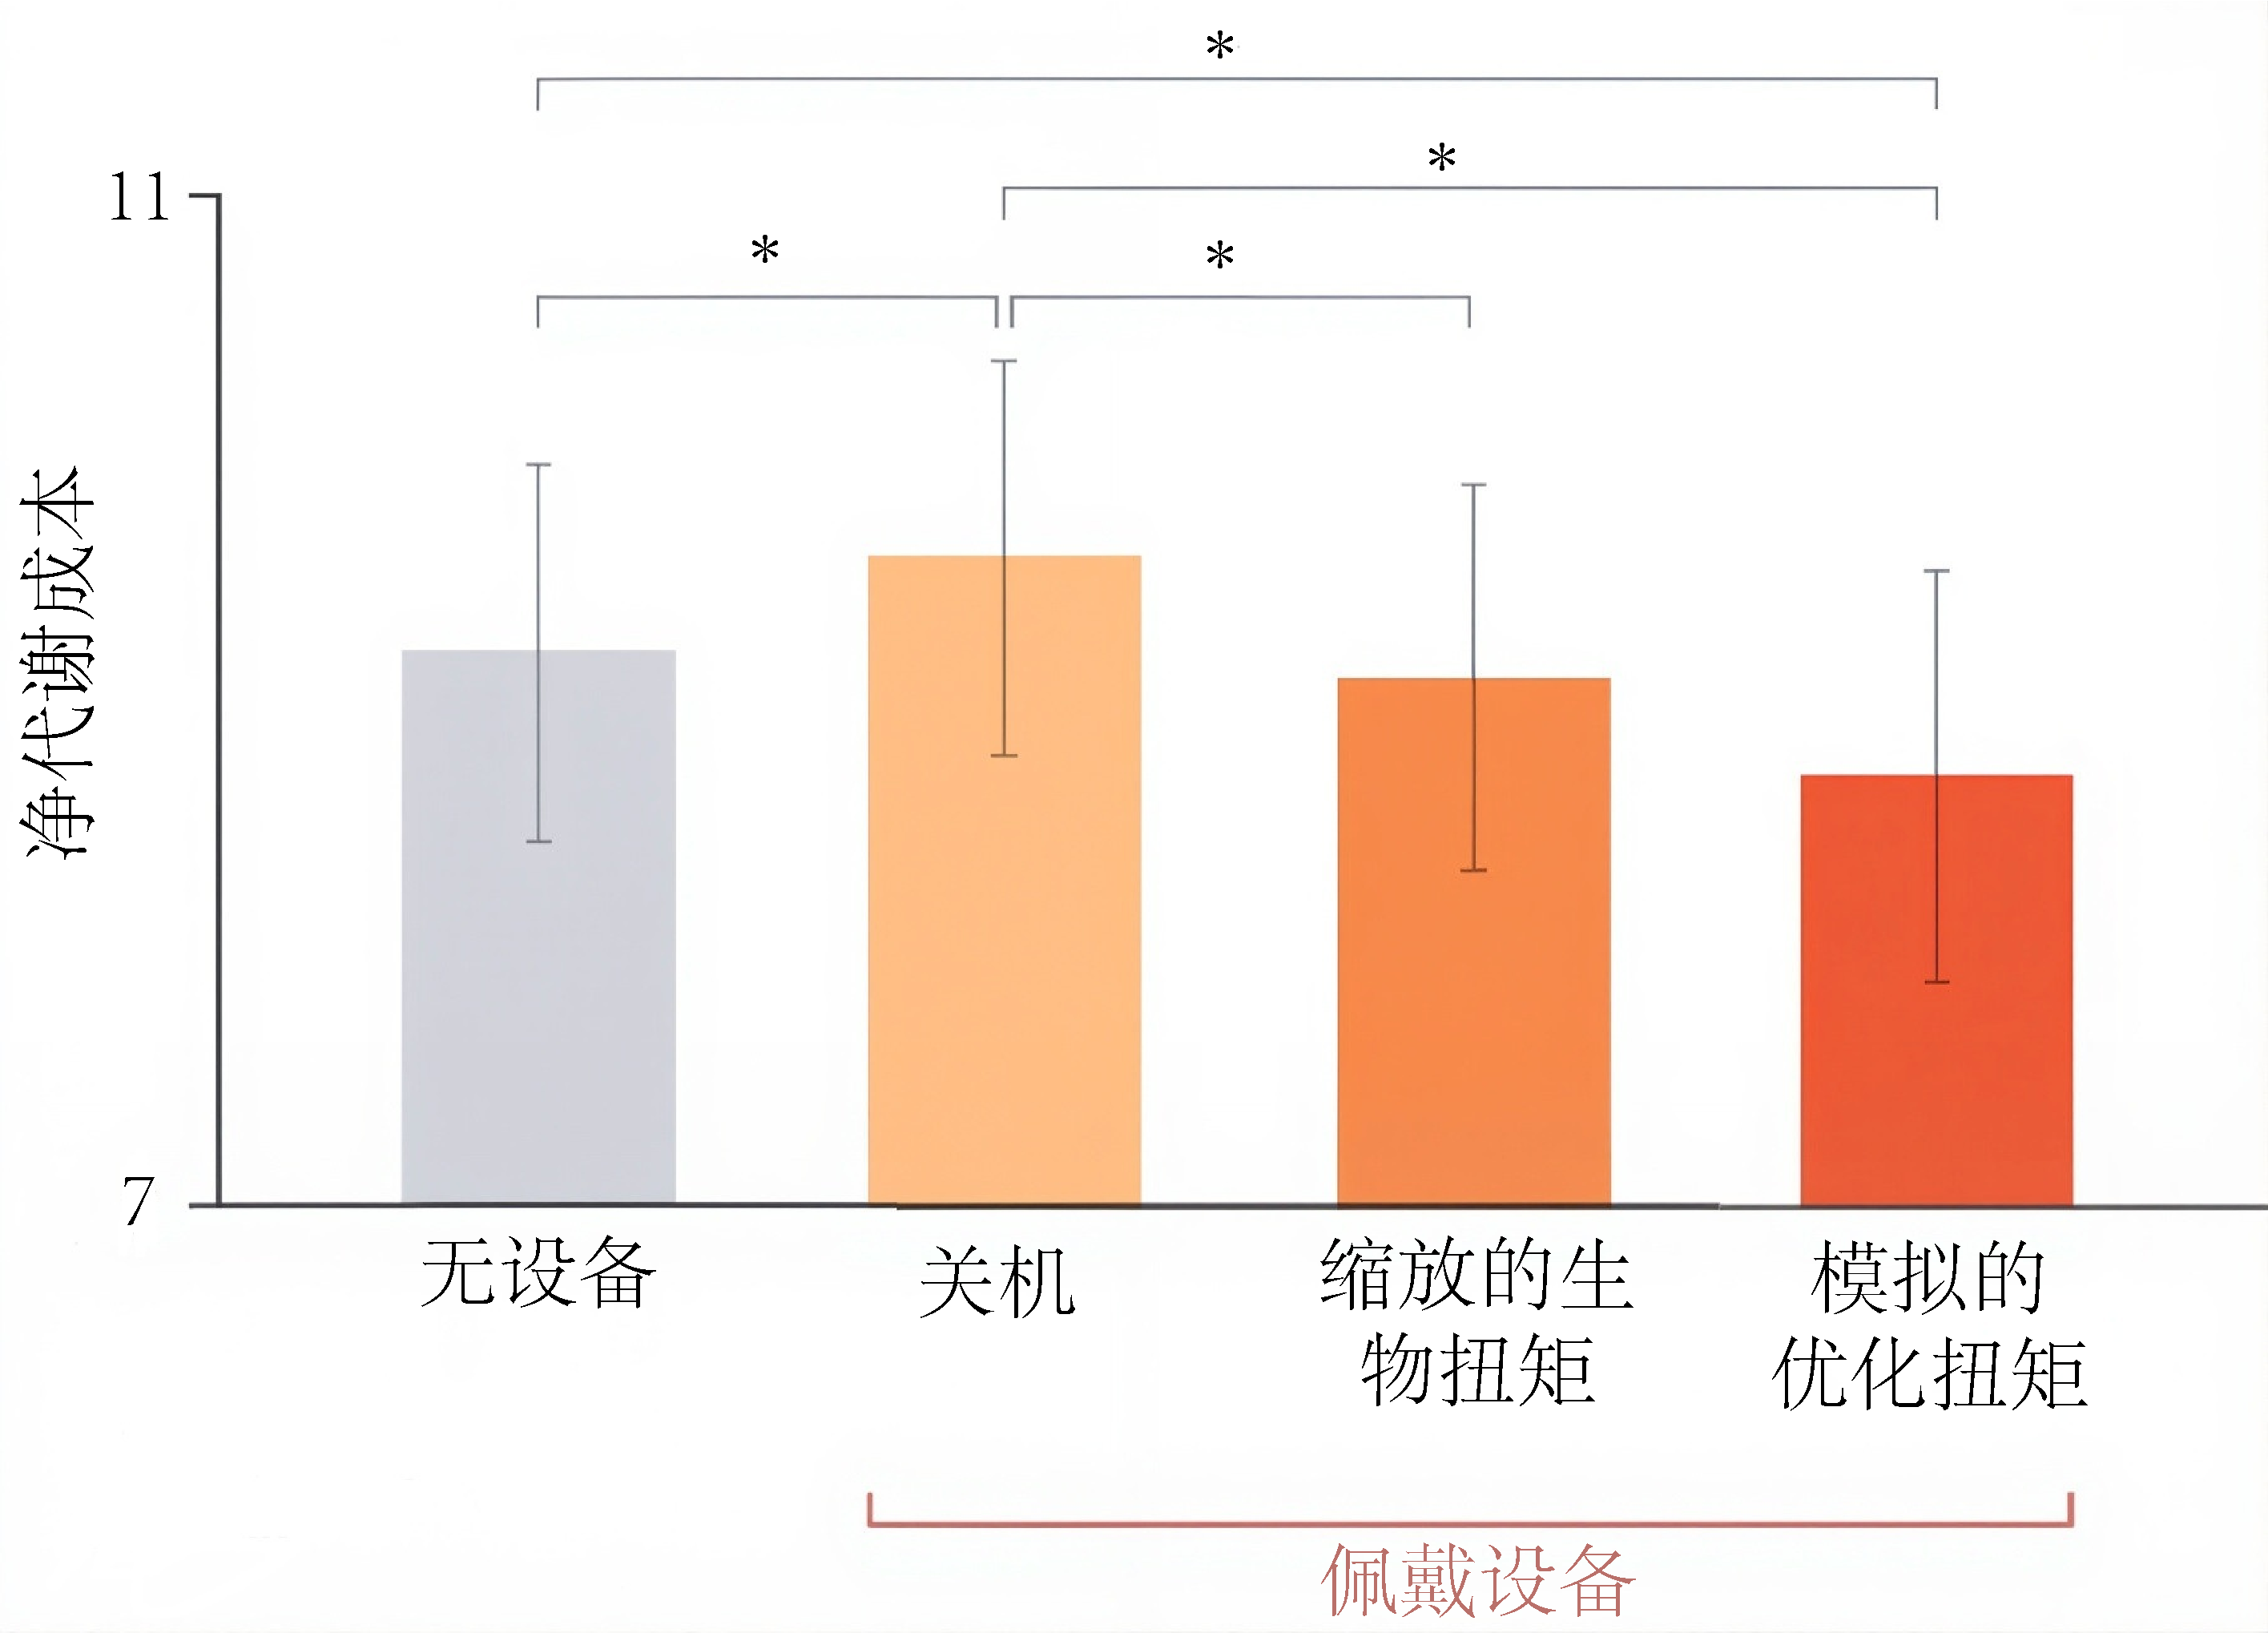
\includegraphics[width=0.65\linewidth]{chap12/12_14}
	\caption{Lee 等人的髋部伸展装置在施加由肌肉驱动模拟而非净关节力矩驱动的扭矩时,能更有效地降低跑步时的代谢成本。
		代谢功率消耗以站立时消耗的功率为基准,经体重标准化,并取 9 名受试者以 2.5 米/秒的速度跑步时的平均值(平均值±1 个标准差;$*p \leq 0.05$)\cite{lee2017reducing}。 \label{fig:12_14}}
\end{figure}


\section{弹簧增强跑步}

艾略特$\cdot$霍克斯是一位跑步爱好者,也是我运动生物力学课程的前学生。
一天下午,他在金门公园骑自行车。
公园的赛道呈同心圆状,内侧为自行车道,外侧为跑步者道。
绕圈骑行很无聊,所以艾略特自然而然地把注意力转向了跑步者。
从自行车的参考系来看,跑步者几乎静止不动(除了他们的腿),就像在固定的树干下来回摆动的钟摆。
艾略特想到,或许可以用弹簧连接跑步者的腿来节省能量。
第二天,艾略特和他的实验室伙伴科尔$\cdot$辛普森(他们也有类似的想法)在鞋子上绑了一些医用管,然后出去跑了一小段。
感觉棒极了。
这次快速的研究激发了一个为期两年的团队项目,探索如何利用这个简单的装置降低跑步的能量消耗。


该团队用乳胶管制作弹簧,并将两端分别固定在跑步者的鞋面上(图~\ref{fig:12_15})。
弹簧必须足够长,以便在双脚交叉时不会产生弹力,并且在双脚分开较远时不会断裂;
同时,弹簧也必须足够短,以免缠绕在一起。
初始装置的刚度为125 N/m,自由长度等于参与者腿长的25\%。
弹簧质量约为 0.02 公斤。
我们测试了许多弹簧,但没有一个比这个初始设计有显著的优势。
学生们绕着斯坦福校园跑了 6 公里,没有绊倒(这最初是一个担忧)。


\begin{figure}[!htb]
	\centering
	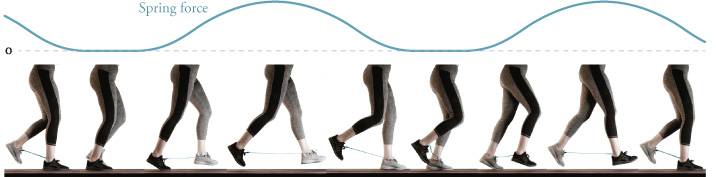
\includegraphics[width=1.0\linewidth]{chap12/12_15}
	\caption{延时摄影:一位跑步者使用弹簧连接双腿以提高跑步效率。
		双腿分开时,弹簧会产生力量。
		图片由卡拉$\cdot$韦尔克提供。 \label{fig:12_15}}
\end{figure}


我们测量了 12 名健康参与者在跑步机上以 2.7 米/秒的速度跑步时的代谢能量消耗,参与者分别穿着和不穿着通过弹簧连接的鞋子。
在两天的测试中,参与者每人完成了 4 次 10 分钟的借助弹簧的跑步,并穿插了 4 次 10 分钟的不使用弹簧的自然跑步作为实验对照。
在第一次试验中,与自然跑步相比,参与者在使用弹簧跑步时没有表现出代谢节省。
然而,到第二次试验结束时,与自然跑步相比,参与者在弹簧辅助跑步期间消耗的能量减少了 3.8 ± 5.4\% (p = 0.034)。
代谢节省随着练习而增加,并且到第二天测试结束时,所有参与者跑步时消耗的能量都减少了。
平均能量节省为 6.4 ± 2.8\% \cite{simpson2019connecting}。


为了探索弹簧降低能量的机制,我们开发了一个OpenSim跑步模型,分别模拟了连接腿部和腿部的弹簧。
模型显示,弹簧产生的力矩作用于髋部和膝部,从而减少了肌肉产生的髋部和膝部力矩(图~\ref{fig:12_16})。
弹簧通过一种复杂的机制提高了跑步的经济性,这种机制产生的能量节省超过了腿部摆动带来的能量节省。
当跑步者学会使用弹簧时,他们会采用步幅更短、步频更高的跑步步态。
更短更快的步幅反过来又减少了站立时重心转移所需的功。
因此,弹簧不仅减少了摆动时的功,也减少了站立时的功。


\begin{figure}[!htb]
	\centering
	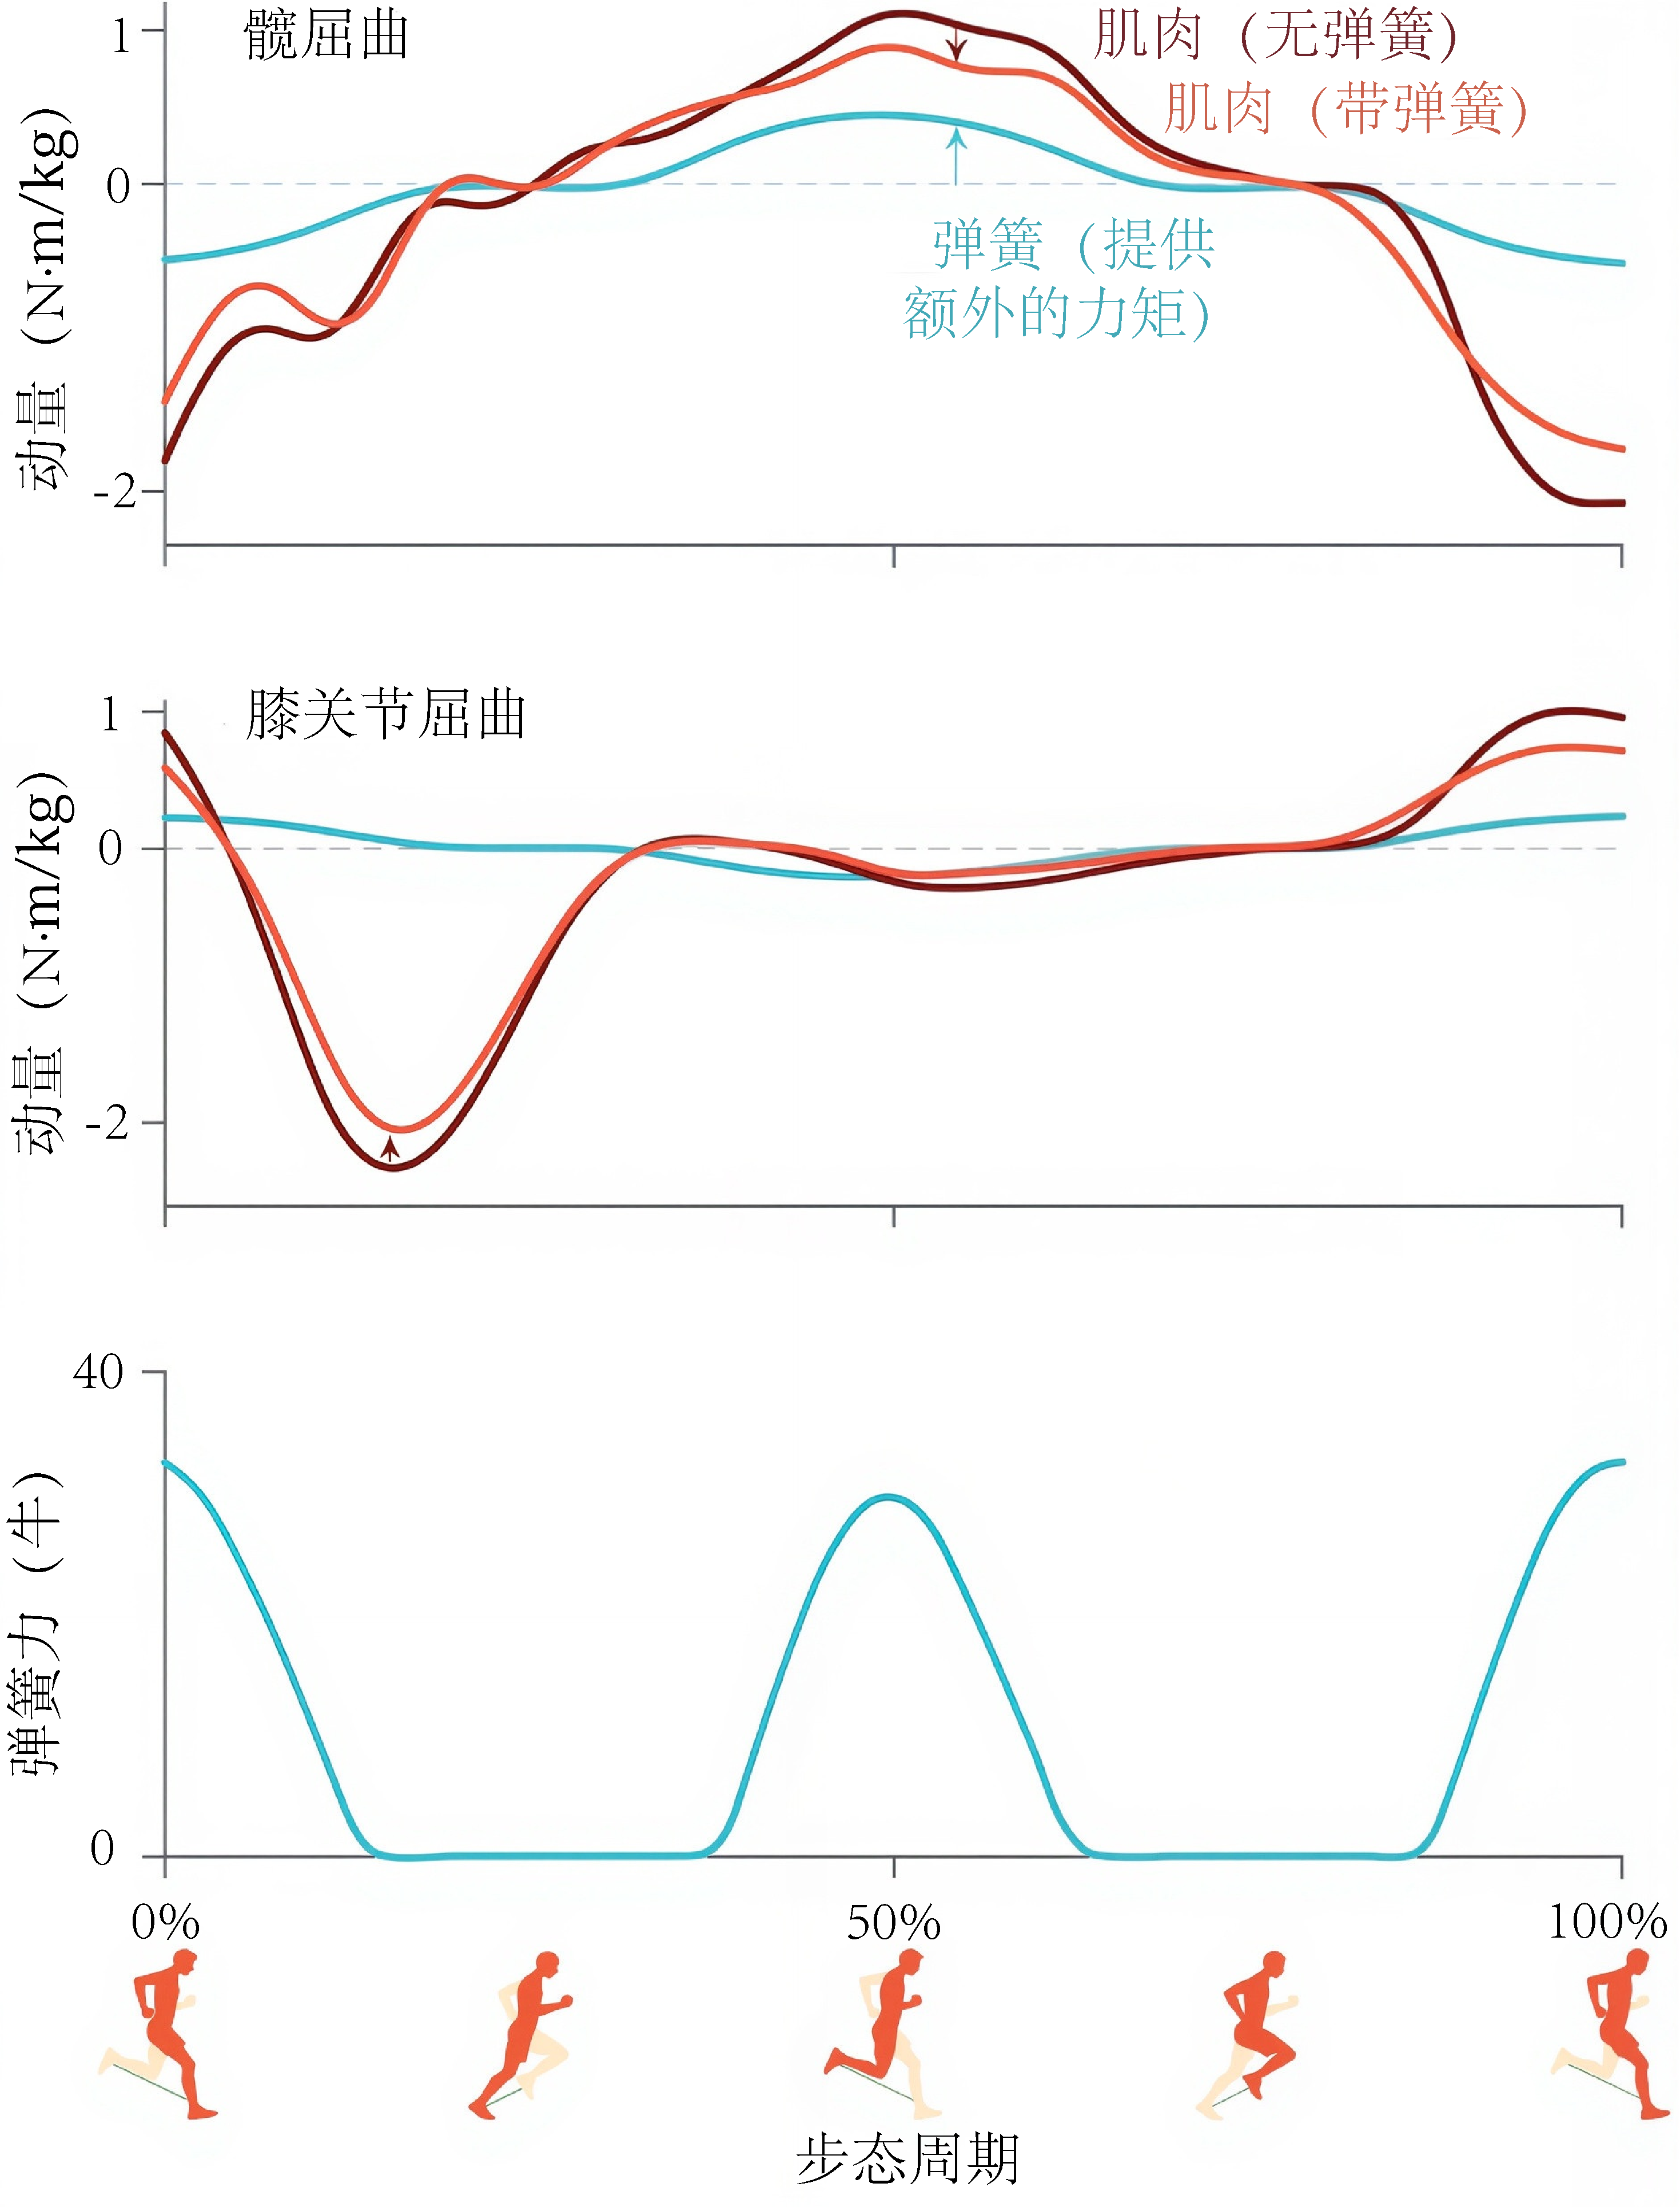
\includegraphics[width=0.75\linewidth]{chap12/12_16}
	\caption{腿部连接弹簧跑步时的能量节省机制。
		由于弹簧的辅助,摆动过程中肌肉产生的力矩减少。
		站立时肌肉产生的力矩也减少,
		这可能是由于步频增加所致\cite{simpson2019connecting}。 \label{fig:12_16}}
\end{figure}


连接双腿的弹簧可以作为一种廉价的辅助装置,提升人类的跑步表现,或者作为一种简单的干预措施,进一步探索人机交互。
艾略特$\cdot$霍克斯在自行车上构思这项发明的经历提醒我们,新的视角可以带来创造性的洞见。
